\documentclass[a4paper, 10pt, twocolumn, DIV=calc]{scrartcl}
\usepackage[T1]{fontenc}
\usepackage[utf8]{inputenc}
\usepackage{arsclassica}
\usepackage{graphicx}
\usepackage{booktabs}
\usepackage{array}
\usepackage{tabularx}
\usepackage{listings}
\usepackage{makecell}
\usepackage{multirow}
\usepackage{colortbl}
% make tables from csv files
\usepackage[l3]{csvsimple}
% subfigures
\usepackage{subcaption}

\usepackage{geometry}
\geometry{top=1cm,bottom=1.5cm,left=2.5cm,right=2.5cm,includehead,includefoot}
\setlength{\columnsep}{7mm}

% less detail on the toc
\setcounter{tocdepth}{2}

\begin{document}
\author{Camilla Maffeis \and Giulia Fabiani}
\title{Data Mining 2 Project}
\date{A.Y. 2024/2025}

%\maketitle

% First page: title + TOC
\begin{titlepage}
    \maketitle
    \vfill
    \tableofcontents
    \vfill
\end{titlepage}
%\twocolumn

\section{Data Understanding and Preparation}
\label{data_understanding}
The goal of this project is to analyze two datasets providing different kinds of information about movies, TV shows, and other forms of visual entertainment.

In the following section, we'll focus on the tabular dataset, while the overview about the time series dataset composition and preparation can be found in Section \ref{time_series_analysis}.

This dataset is an extension of the one proposed in DM1: the records include key information about titles, insights into critical aspects such as awards and reviews, as well as ratings and further data about the title's production.

\subsection{Data Semantics, Duplicates and Train/Test Split}

The tabular dataset contains 149,531 records and 32 attributes; the nine attributes that were added to the original set from the DM1 dataset are reported in Tab. {\ref{tab:original_feats}}. This makes a total of nine categorical attributes, three binary attributes and 20 numerical attributes. Among the latter, only \textit{runtimeMinutes} and \textit{averageRating} can be classified as continuous, as the others mostly represent counts.

A first data quality check revealed only ten genuine duplicates, i.e. records sharing all feature values, which we dropped.

We then split the dataset, reserving 70\% for training, and the remaining 30\% for testing. As to avoid data leakage, we performed all subsequent data exploration exclusively on the training set. At the end of the data preparation stage, we applied all transformation and cleaning steps to the test set as well.

\begin{table*}
    \centering
    \renewcommand{\arraystretch}{1.2}
    \scriptsize
    \rowcolors{2}{}{gray!25}
    \begin{tabular}{p{3cm}p{7.5cm}p{3cm}}
        \toprule
        \textbf{Feature} & \textbf{Description} & \textbf{Type} \\ \midrule
        castNumber & Total Number of Cast individuals present within the IMDb title page. & Discrete. Ratio-scaled. \\
        companiesNumber & Total Number of companies that worked for the title. & Discrete. Ratio-scaled. \\
        regions & The regions for this version of the title. Some titles can belong to more than one class. & Categorical. 171 unique classes. \\
        averageRating & Weighted average of all the individual user ratings. & Continuous. Ratio-scaled. \\
        externalLinks & Total Number of External Links the title has within the IMDb page. & Discrete. Ratio-scaled. \\
        quotesTotal & Total Number of quotes the title has within the IMDb page. & Discrete. Ratio-scaled. \\
        writerCredits & Total number of writer credits of the title. & Discrete. Ratio-scaled. \\
        directorCredits & Total number of director credits of the title. & Discrete. Ratio-scaled. \\
        soundMixes & Technical specification of the sound mixes available for the title. Some titles can belong to more than one class. & Categorical. 59 unique classes. \\
        \bottomrule
    \end{tabular}
    \caption{New features in the extended dataset.}
    \label{tab:original_feats}
\end{table*}

\subsection{First Global Exploration of the Training Set}
A first global analysis of the dataframe's summary and descriptive statistics revealed missing values for \textit{endYear} (100,729), \textit{runtimeMinutes} (28,185), \textit{countryOfOrigin} (27,961) and \textit{genres} (1,887). Since most records are missing an \textit{endYear}, and the feature is strongly correlated to \textit{startYear}, we dropped it.

Since a great majority of records had no information about sound mixes, we decided to drop this feature as well.

\textit{bestRating}, \textit{worstRating}, and \textit{isRatable} were once again confirmed to be uninformative, as they only take one value for all records (10, 1, and 1, respectively), and were therefore dropped. We also dropped \textit{ratingCount}, as it was strongly correlated to \textit{numVotes}, and \textit{isAdult}, because it's redundant w.r.t. the \textit{adult} category in \textit{genres}.

Checking the values for the only remaining original binary attribute, \textit{canHaveEpisodes}, we noticed that only two records with a \textit{titleType} different from \textit{tvSeries} and \textit{tvMiniSeries} have a positive value. We corrected them: the first had been registered as a \textit{tvMovie} instead of \textit{tvSeries}, while the second was a short with no episodes.

Lastly, we removed the string \texttt{'\textbackslash \textbackslash N'}, which was prepended to all lists of \textit{regions}, making the feature consistent with \textit{numRegions}.


\subsection{Distribution of Categorical Variables and Statistics}

\begin{figure}
    \centering
    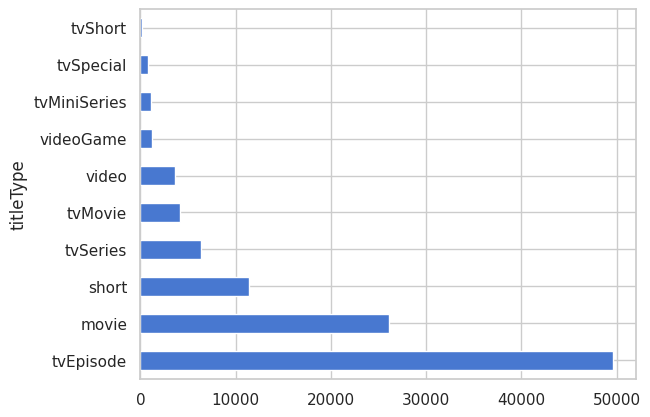
\includegraphics[width=\columnwidth]{../results/images/titleType_distribution.png}
    \caption{Distribution of \textit{titleTypes}.}
    \label{fig:titleType_distribution}
\end{figure}

\begin{figure}
    \centering
    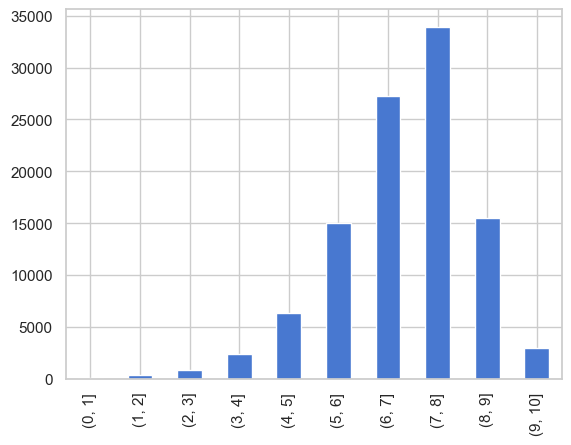
\includegraphics[width=\columnwidth]{../results/images/rating_distribution.png}
    \caption{Barplot for \textit{rating}.}
    \label{fig:rating_histogram.png}
\end{figure}

In this subsection, we studied the univariate and bivariate distribution of categorical variables, which all turned out to be unbalanced.

Differently from the DM1 dataset, the most popular \textit{\textbf{titleType}} is \textit{tvEpisode} (47\% of the records), followed by \textit{movie} (25\%) and \textit{short} (11\%); \textit{tvSpecial} (0.79\%) and \textit{tvShort} (0.17\%) are the classes with the lowest support (cf Fig \ref{fig:titleType_distribution}). With regard to \textit{\textbf{genres}}, the two most popular classes are by far \textit{Drama} and \textit{Comedy}, although it depends on \textit{titleType}.
Binned \textit{\textbf{rating}} follows a left-skewed distribution, with the mode being the [7,8) class (Fig. \ref{fig:rating_histogram.png}).
The most popular \textit{\textbf{countryOfOrigin}} and \textit{\textbf{region}} is the US, but both features have a substantial amount of missing values: \textit{nan} is the second most popular value for both.

We dropped \textit{soundMixes}: not only are most of its 59 unique values very rare, it has too many missing values to provide useful information.


\subsection{Distribution of Numeric Variables and Statistics}
\label{numeric_vars_analysis}
Before analyzing numeric variables, we added the same features we had added to the DM1 dataset:
\begin{itemize}
    \item \textit{numCountriesOfOrigin}: the number of countries listed for the record for the variable \textit{countryOfOrigin}. For the training set, the values range from 1 to 10.
    \item \textit{numGenres}: the number of genres listed in \textit{genres}. For the training set, the values range from 1 to 3.
    \item \textit{reviewsTotal}: the sum of \textit{criticReviewsTotal} and \textit{userReviewsTotal}.
    \item \textit{criticReviewsRatio}: the proportion of review from critics (\textit{criticsReviewTotal}) on the total number of reviews of a record (\textit{reviewsTotal}). For unreviewed records, it is set to zero.
    \item \textit{awardsAndNominations}: the sum of \textit{awardWins} and \textit{awardNominationsExcludeWins}.
\end{itemize}

A pairplot of all numeric variables, with KDE graphs on the diagonal, allowed us to gain a global view of both the features' univariate distribution and their pairwise correlations. Given the size of the dataset, we resorted to using a random sample of 20,000 records.
The great majority of the variables has a right-skewed distribution (\textit{writerCredits, numRegions, awardWins, totalImages, criticReviewsTotal, runtimeMinutes, userReviewsTotal, totalCredits, totalVideos, castNumber, numVotes, quotesTotal, awardNominationsExcludeWins, companiesNumber, externalLinks, awardsAndNominations, numCountriesOfOrigin, reviewsTotal}).
\textit{averageRating}, of course, follows the same left-skewed distribution observed for its discretized version, \textit{rating} (cf. Fig. \ref{fig:rating_histogram.png}).

We observed that some records have an implausibly long runtime, probably due to the inconsistent strategy adopted for the computation of the runtime for serialized content, for which sometimes the total runtime of a series is registered, rather than the average episode runtime.
In order to avoid this problem, we removed the runtime of all \textit{tvSeries}, \textit{tvMiniSeries}, and \textit{tvEpisodes} for which the value exceeded the 3rd quartile + 1.5 interquartile range for its specific category (105, 382.5 and 84 minutes, respectively); a total of 1560 records in the training set were affected.

A similar problem was found for \textit{writerCredits}: records with suspiciously high values are likely TV episodes for which all writers of the entire TV series were erroneously credited.
Therefore, we decided to remove the values for \textit{writerCredits} from 2100 \textit{tvEpisodes}, as they exceeded the 3rd quartile + 1.5 interquartile range (8.5 credits).

\subsection{Variable Transformation, Pairwise Correlations and Elimination of Variables}
We log-transformed all right-skewed variables, and used the Shapiro-Wilk test to determine whether they now resembled a normal distribution. None of them did, therefore we used Spearman's correlation coefficient in our correlation analysis.

% \begin{figure}
%     \centering
%     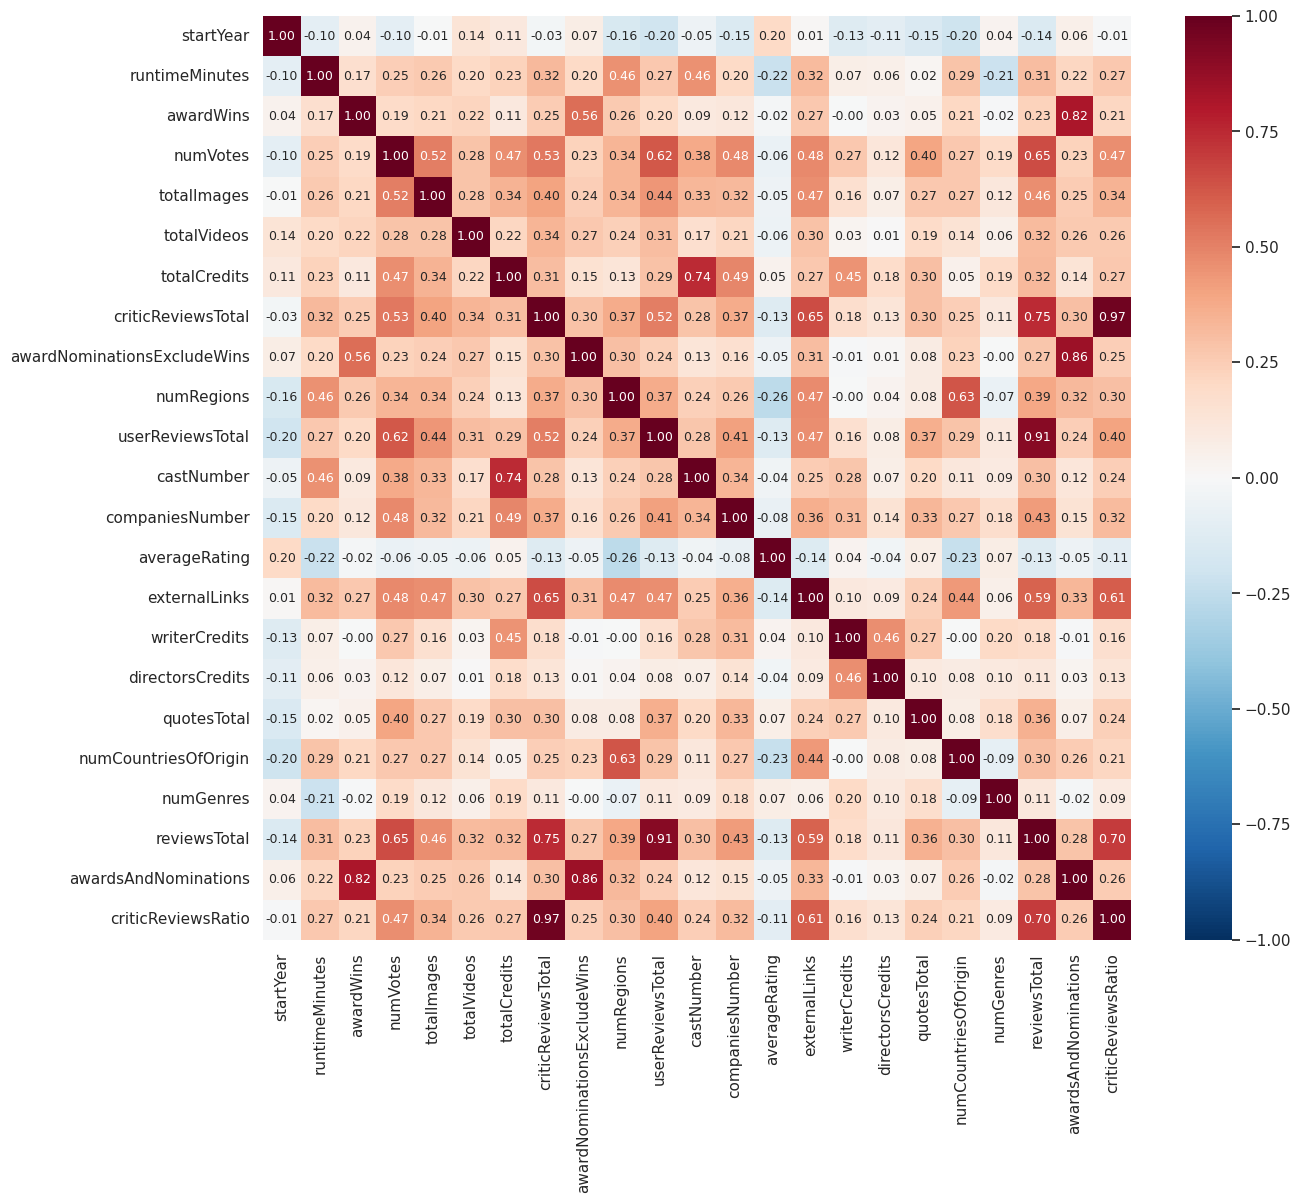
\includegraphics[width=\columnwidth]{../results/images/corr_heatmap_before.png}
%     \caption{Correlation heatmap before attribute removal.}
%     \label{fig:corr_heatmap_before.png}
% \end{figure}

We removed the following features because they were highly correlated to another feature: \textit{awardNominationsExcludeWins} (0.86, correlated with \textit{awardsAndNominations}), \textit{castNumber} (0.74, with \textit{totalCredits}).
Since all features regarding reviews and \textit{numVotes} were highly correlated with each other, we dropped them all with the exception of \textit{numVotes}, which has the least skewed distribution, and \textit{criticReviewsRatio}, which offer insights of a different nature. We however decided to conserve information about the presence/absence of reviews by users and critics with the creation of two new boolean features: \textit{hasUserReviews} and \textit{hasCriticsReviews}.

Moreover, we binarized features which overwhelmingly took on the value 0 (or 1, in the case of \textit{numCountriesOfOrigin} and \textit{directorsCredits}). The results of these transformations are reported in Table \ref{tab:binarized_features}.

\begin{table}
    \centering
    \small
    \setlength{\tabcolsep}{6pt}
    \renewcommand{\arraystretch}{1.1}
    \rowcolors{2}{}{gray!25}
    \begin{tabular}{l l c}
    \toprule
    \textbf{Original feature} & \textbf{Boolean version} & \textbf{\% True} \\
    \midrule
    awardWins            & hasAwards                       & 8.16  \\
    \makecell[l]{awardsAnd \\ Nominations}
                         & \makecell[l]{hasAwardsOr \\ Nominations} & 12.25 \\
    totalVideos          & hasVideos                       & 7.93  \\
    criticReviewsTotal   & hasCriticsReviews               & 24.88 \\
    userReviewsTotal     & hasUserReviews                  & 36.98 \\
    \makecell[l]{directors \\ Credits}
                         & \makecell[l]{moreDirectors \\ Credits} & 9.89  \\
    quotesTotal          & hasQuotes                       & 13.86 \\
    \makecell[l]{numCountries \\ OfOrigin}
                         & \makecell[l]{moreCountries \\ OfOrigin} & 5.05  \\
    \bottomrule
    \end{tabular}
    \caption{Binarization of numeric features.}
    \label{tab:binarized_features}
\end{table}


The total number of final features is 27; they are listed in Tables \ref{tab:dataset_numeric} and \ref{tab:dataset_categorical}. Among the remaining numeric features, the heatmap in Fig. \ref{fig:corr_heatmap_after.png} shows that \textit{externalLinks} exhibits a moderate to high positive correlation with \textit{criticReviewsRatio} (0.61) and a low to moderate correlation with \textit{numRegions}, \textit{numVotes} and \textit{totalImages} (around 0.47), while \textit{numVotes} is also mildly correlated to \textit{totalImages}, \textit{totalCredits}, \textit{criticReviewsRatio}, and \textit{companiesNumber} (between 0.47 and 0.52).

\begin{figure}
    \centering
    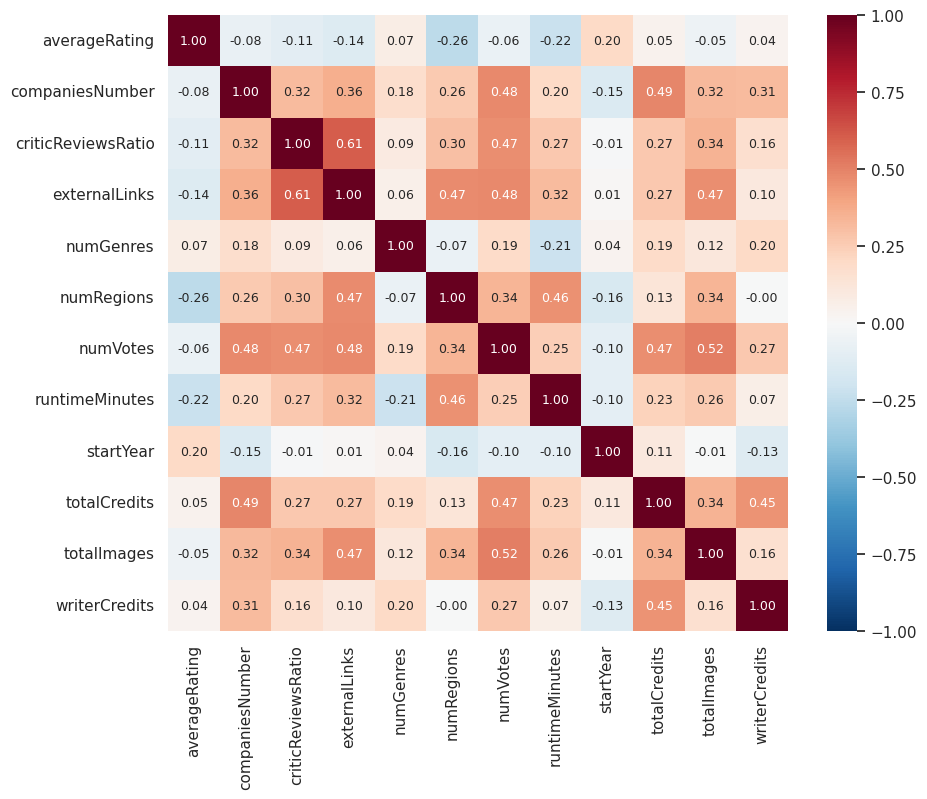
\includegraphics[width=\columnwidth]{../results/images/corr_heatmap_after.png}
    \caption{Correlation heatmap after attribute removal.}
    \label{fig:corr_heatmap_after.png}
\end{figure}


\begin{table*}[t]
    \centering
    \renewcommand{\arraystretch}{1.2}
    \scriptsize
    \rowcolors{2}{}{gray!25}
    \begin{tabular}{p{2.5cm}p{7cm}p{4.5cm}}
    \toprule
    \textbf{Feature} & \textbf{Description} & \textbf{Type} \\
    \midrule
    runtimeMinutes & Primary runtime of the title, in minutes. & Continuous. Ratio-scaled. \\
    startYear & Represents the release year of a title. In the case of TV Series, it is the series’ start year. & Discrete. Interval. \\
    numVotes & Number of votes the title has received. & Discrete. Ratio-scaled. Log-transformed. \\
    numRegions & The regions number for this version of the title. & Discrete. Ratio-scaled. Log-transformed. \\
    totalImages & Total number of images for the title within the IMDb title page. & Discrete. Ratio-scaled. Log-transformed. \\
    totalCredits & Total number of credits for the title. & Discrete. Ratio-scaled. Log-transformed. \\
    criticReviewsRatio & The proportion of reviews from critics on the total number of reviews of a record. For unreviewed records, it is set to 0. & Continuous. Ratio-scaled. \\
    numGenres & The number of genres listed for the variable \textit{genres}. & Discrete. Ratio-scaled. \\
    companiesNumber & Total number of companies that worked for the title. & Discrete. Ratio-scaled. \\
    externalLinks & Total number of external links the title has within the IMDb page. & Discrete. Ratio-scaled. \\
    writerCredits & Total number of writer credits of the title. & Discrete. Ratio-scaled. \\
    averageRating & Weighted average of all the individual user ratings. & Continuous. Ratio-scaled. \\
    \bottomrule
    \end{tabular}
    \caption{Numeric attributes after data preparation.}
    \label{tab:dataset_numeric}
\end{table*}

\begin{table*}[t]
    \centering
    \renewcommand{\arraystretch}{1.2}
    \scriptsize
    \rowcolors{2}{}{gray!25}
    \begin{tabular}{p{2.5cm}p{7cm}p{4.5cm}}
    \toprule
    \textbf{Feature} & \textbf{Description} & \textbf{Type} \\ \midrule
    originalTitle & Original title, in the original language. & Categorical; mostly unique classes (i.e. names). \\
    titleType & The type/format of the title (e.g. movie, short, tvseries, tvepisode, video, etc.). & Categorical, 10 classes. \\
    countryOfOrigin & The country where the title was primarily produced. & Categorical, 153 classes. Some titles can belong to more than 1 class. \\
    genres & The genre(s) associated with the title (e.g., drama, comedy, action). & Categorical, 29 classes. Some titles can belong to more than 1 class. \\
    regions & The regions for this version of the title. & Categorical, 171 unique classes. Some titles can belong to more than 1 class. \\
    rating & IMDB title rating class. & Ordinal, 10 values. \\
    hasAwards & Whether the title has won at least an award & Asymmetric binary. \\
    hasAwardsOrNominations & Whether the title was at least nominated for an award. & Asymmetric binary. \\
    canHaveEpisodes & Whether the title can have episodes. & Asymmetric binary. \\
    hasVideos & Whether the title IMDb title page has at least one video. & Asymmetric binary. \\
    moreCountriesOfOrigin & Whether the title was produced in more than one country. & Asymmetric binary. \\
    hasCriticsReviews & Whether the title has any critic reviews. & Asymmetric binary. \\
    hasUserReviews & Whether the title has any user reviews. & Asymmetric binary. \\
    moreDirectorsCredits & Whether the title has more than one director credits. & Asymmetric binary. \\
    hasQuotes & Whether the title has any quotes within the IMDb page. & Asymmetric binary. \\ \bottomrule
    \end{tabular}
    \caption{Categorical, ordinal, and binary attributes after data preparation.}
    \label{tab:dataset_categorical}
\end{table*}




\subsection{Handling Missing Values}
\label{handling_nan}
At this point, we still have missing values for \textit{countryOfOrigin}, \textit{region}, \textit{genres}, \textit{runtimeMinutes} and \textit{writerCredits}; some were preexisting, others were removed as detailed Subsec. \ref{numeric_vars_analysis}.
Since the distribution of \textit{runtimeMinutes} depends on \textit{titleType}, and the same holds true for \textit{writerCredits}, we imputed their missing values using the median value within each respective class.

On the other hand, we chose not to replace missing values for \textit{genres}, \textit{region} or \textit{countryOfOrigin}. They can easily be handled when performing the encoding for our methods without introducing bias, therefore we'd rather preserve the original distributions and correlations.


\subsection{Clustering}\label{sec:tabular_clustering}
\begin{figure*}
    \center
    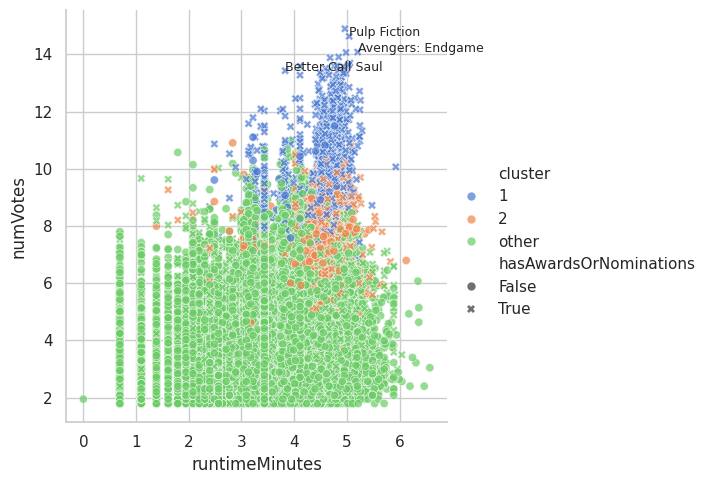
\includegraphics[width=.8\textwidth]{../results/images//understanding_clustering.png}
    \caption{Hierarchical clustering results on tabular data by runtime and number of votes.}
    \label{fig:tabular_clustering}
\end{figure*}

As part of the data understanding phase, we conducted hierarchical clustering on the dataset, using all numeric attributes.

Since the size of the dataset made it unfeasible to perform hierarchical clustering directly because of the computational cost of computing distances between all records, we firstly reduced our dataset to a more manageable 10,000 records, running k-means clustering with k=10,000.

We then performed hierarchical clustering on the centroids of K-Means clusters, experimenting with different linkage methods and inspecting the resulting dendrograms. We found that using average linkage yielded the most satisfactorily results. We then cut the dendrogram at an appropriate threshold and, after propagating cluster labels back to the entire dataset, analyzed the composition of the clusters.

We found 13 clusters of varying sizes, with the top cluster grouping one fifth of the entire dataset and the top four clusters grouping half of the dataset. Five clusters contained less than 5,000 records each.

For reasons that will become apparent in \ref{sec:anomaly_detection}, we concentrated our analysis on two smaller clusters: C1 (1,668 records) and C2 (3,923). These clusters belong to the same supercluster, that is merged latest of all with the rest of the dataset.

Both clusters are made up primarily from movies (with some tv series), and according to their distribution w.r.t. \emph{numVotes}, probably contain blockbuster movies and very popular TV series \ref{fig:tabular_clustering}.
In addition to that, almost 57\% of records from C1 received awards, a proportion that increases to 80\% when considering also nominations.
C2 records were also well received, with 45\% of them having received or being considered for awards.
In addition to that, 87\% of records from C1 and 45\% of records from C2 have videos on their IMDB page and almost all records from both C1 and C2 have both reviews from users and from critics.

\section{Advanced Data Pre-Processing}
\subsection{Anomaly detection}\label{sec:anomaly_detection}
\subsection{Imbalanced Learning}

In this section we with several imbalance learning techniques in the context of binary classification.
Our goal was to develop a system that is capable of predicting which titles have received any awards (as already seen in \ref{tab:binarized_features}, only about 8\% our training records did).
We figured that a similar system could be useful in a number of contexts, like for recommendation and showcasing purposes or for streaming platforms attempting to decide which titles to license when this information isn't already available (for example for newly released titles).

\subsubsection{Resampling techniques}

We established a performance baseline using a KNN classifier with no resampling techniques.
We then experimented with three over-sampling strategies (Random Over-sampling, SMOTE, ADASYN), two under-sampling strategies (Random Under-sampling and Edited Nearest Neighbors) and a combination of both (SMOTEEN). In all cases we resampled the dataset as to obtain a perfect balance between the positive and the negative class.

For each technique we fine tuned the hyperparameters of the classifier searching for the best F1 score: initially we performed random seach on ks between 1 and 100, with euclidean and manhattan distance, both weighting neighbors and not. Since we noticed generally better performance with weighting of exemplars, we removed unweighted models from the grid search.

We also noticed that for over-sampling methods performance was rapidly decreasing as k  got bigger, so we restricted our grid search to odd ks between 1 and 21. Since performance of under-sampling techniques wasn't degrading so rapidly, we extended the number of neighbors considered for these approaches to odd numbers between 1 and 41, but we noticed that scores were nevertheless plateauing around 10, so we didn't consider it necessary to widen the search beyond that.

We then compared performance of different resampling strategies checking precision, recall and F1 score on 5-fold cross validation (cf \ref{tab:imb_learn_cv_performance}).

\begin{table}
    \footnotesize
    \csvautobooktabular{../results/tables/imb_learn_cv_performance.csv}
    \caption{Results of tested resampling methods on 5-fold cross validation.}
    \label{tab:imb_learn_cv_performance}
\end{table}

Precious insights were also gathered by the inspection of the precision-recall curves (reported in fig \ref{fig:imb_learn_cv_pr}) and average precision.

\begin{figure*}
    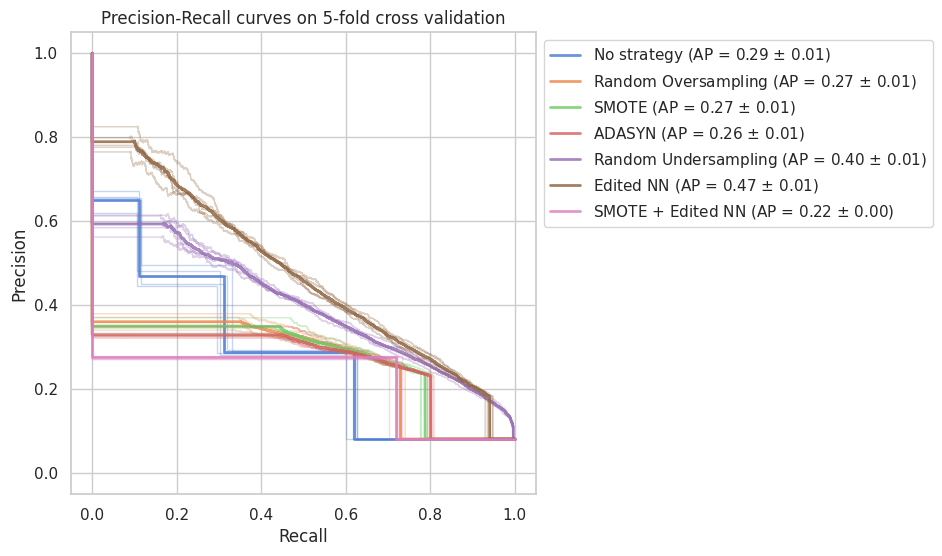
\includegraphics[width=.8\textwidth]{../results/images/imb_learn_cv_pr.png}
    \caption{Precision-Recall curves on 5-fold cross-validation for different resampling methods}
    \label{fig:imb_learn_cv_pr}
\end{figure*}

Over-sampling methods and the combination of SMOTE and Edited NN all show worse ranking capabilities than no resampling strategy at all. In particular these methods demonstrate much worse performance in the early retrieval range of operating points, meaning that they have much more false positives in the top ranked instances.
This is also reflected in the lower precision scores that are not balanced by the higher recall.
In addition to that, over-sampling techniques, even when relatively inexpensive at fitting time (Random Over-sampling), are slower at prediction time (because of the necessity to compute distances with all records in the over-sampled dataset) and have considerably higher space requirements.

Performance obtained with Random Under-sampling has similar F1 score to no resampling strategy, but shows better ranking capabilities, as demonstrated both by AP score and inspection of the PR curve.

The best results are obtained with Edited Nearest Neighbor. The PR curve for ENN almost always dominates random under-sampling with minimal crossing-over for higher values of recall.

It seems to us that Random Under-sampling may be the preferred choice in some context in which fitting time would be a more pressing concern than the precision of the prediction, so we decided to assess both Edited NN and Random Under-sampling on the test set.

\subsubsection{Decision threshold and assessment}
Edited Nearest Neighbor showed satisfactory performance, improving by 0.1 the F1 score of the vanilla KNN and having the best precision among all tested methods (0.50) and recall at least better than the vanilla KNN.
Nevertheless, we decided to post-tune the decision threshold of both our best performing models before assessment on the test set.
For the pipeline using Random Under-sampling this resulted in setting a higher threshold (0.77), while for Edited NN the threshold had to be lowered to 0.38.
Fig \ref{fig:imb_learn_threshold} illustrates the effect of changing the decision threshold for the pipeline using Random Under-sampling: we can observe that at the default threshold the model would have better recall but much worse precision than at the tuned threshold.

\begin{figure}
    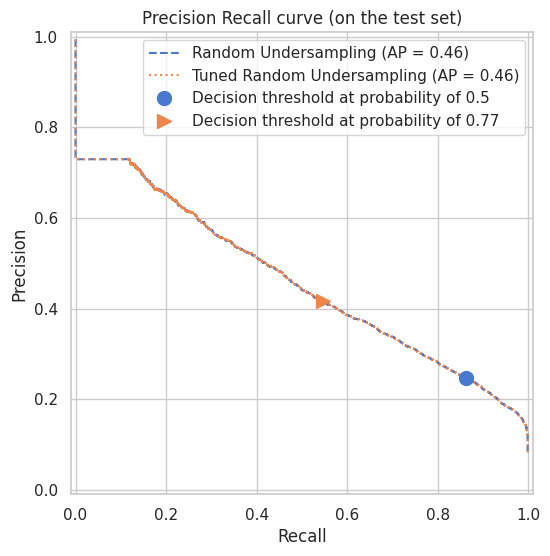
\includegraphics[width=\columnwidth]{../results/images/imb_learn_threshold.png}
    \caption{Decision threshold for KNN with Random Under-sampling before and after tuning.}\label{fig:imb_learn_threshold}
\end{figure}

We finally assessed both models on the test set, obtaining very similar results: ENN obtained a F1 score of 0.49, while Random Under-sampling 0.47; inspecting the other metrics we can confirm that the worse performance of Random Under-sampling is entirely due to a lower precision (0.42 vs 0.44 for ENN), as we had expected from the inspection of the PR curves in validation.


\section{Advanced Classification}
In this section, we  will examine the performance of various advanced classification methods w.r.t two multiclass classification tasks, aiming to predict the \textit{rating} class and the \textit{titleType} of our records.

Since no features showed high correlation with \textit{averageRating}, while some did exhibit different distribution tendencies w.r.t. \textit{titleType}, we anticipated that the second classification task would yield better results.

In evaluating and comparing our classification models, we selected macro F1 as the main performance metric, given that the different target classes have variable support. For each model, we additionally plotted the Precision-Recall (PR) curves for each class using the one-vs-rest strategy and reported its PR AUC. We favored PR curves instead of ROC curves because they are more informative in multiclass and imbalanced settings.

\subsection{Pre-processing}
\label{classification_preprocessing}
For each model, we built a pipeline which proceeded to first preprocess the data (we used the training and test set, cleaned and prepared as detailed in Sec. \ref{data_understanding}) and then pass it to the model, in order for it to be fitted on the training set or applied on the test set.

The preprocessing step included scaling the numerical features, if required by the method, and one-hot encoding the categorical variables. For both tasks, we of course dropped the target variable, including \textit{averageRating} for the rating task.

For \textit{countryOfOrigin} and \textit{region}, we only kept the 25 most frequent countries, aggregating the rest into an \textit{Other} category, to reduce dimensionality. For the MultiLayerPerceptron Classifier (and, later, for the regression task), we further reduced dimensionality, keeping only the top nine countries for both features and dropping \textit{hasAwards} on the account of its positive correlation to \textit{hasAwardsOrNominations}, in order to further reduce computational costs and training time during hyperparameter tuning. 


\subsection{Logistic Regression}
As a baseline, we first tried a Logistic Regression model. As the algorithm assumes that the features follow a Gaussian distribution, we scaled numerical features using PowerTransformer, which reduces skewness and stabilizes variance.

\subsubsection{Rating}
Using the default parameters yielded a macro F1 of 0.144 and an accuracy of 0.388. We performed a grid search using 5-fold cross validation, which resulted in a very small increase, with a 0.146 average macro F1 on the validation sets and 0.152 on the training set, which at least proves no overfitting.
We tested the following hyperparameters (the values for the final model are in bold):
\begin{lstlisting}[basicstyle=\footnotesize\ttfamily,
                   escapeinside={(*@}{@*)}]
  { 'penalty': [(*@\textbf{'l2'}@*), 'l1', 'elasticnet'],
    'C': [0.001, 0.01, 0.1, 1, (*@\textbf{10}@*), 100],
    'l1_ratio': [0.1, 0.3, 0.5, 0.7, 0.9],
    'solver': ['lbfgs', 'sag', 'saga', 'newton-cg',
        (*@\textbf{'newton-cholesky'}@*), 'liblinear']  }
\end{lstlisting}

On the test set, the final model achieved a \textbf{macro F1} of\textbf{ 0.145} and an \textbf{accuracy} of \textbf{0.388}, comparable to the default model. The poor performances across decision thresholds are confirmed by the \textbf{PR AUC} of only \textbf{0.193}.

The model has managed to generalize some information only for the classes with the highest support: the performances peak for the mode, (7,8] (F1: 0.544), its neighboring classes are confused for it most of the time, and as we move to the tail of the bell distribution, it achieves consistently poor results (F1 < 0.05).

Looking at the model's coefficients, the overall most important feature is \textit{hasCriticReviews} (mean absolute value > 1.2, while for the other coefficients in the top 15 is in the interval [0.6, 0.7]): it is the first or second-biggest coefficient for the best performing classes (i.e. for the interval (5,8]), and for all of them it takes on a negative value, i.e. having critical reviews lowers the probability of a record of having an 'average' rating.

\subsubsection{Title Type}
For this task, the final model resulting from the grid search achieved an average validation macro F1 of 0.653 (on the training set: 0.664). The final parameters chosen were: \texttt{{'C': 100, 'penalty': 'l2', 'solver': 'newton-cg'}}.

On the test set, the model achieved a \textbf{macro F1} of \textbf{0.649} and an accuracy of \textbf{0.908}; the improvement w.r.t. the default parameters (0.647 and 0.908) is, again, quite small. The \textbf{PR AUC} is \textbf{0.704}; the curve for each class reflects its performance.

Given that both tasks have 10 target classes, our intuition about \textit{titleType} yielding better results is confirmed.

The four most popular classes (\textit{tvEpisode}, \textit{short}, \textit{movie}, \textit{tvSeries}) achieve great results, with F1 > 0.9. The best performing and most popular class, \textit{tvEpisode}, peaks with 0.978. All other classes (except \textit{tvShort}) achieve a F1 score > 0.4, which is still significantly more than random chance. \textit{Videogame}, in spite of its low support, manages to achieve very good results (F1 0.76).

The 15 most important features are reported in Fig. \ref{fig:LR_feat_impo_tt.png}. Overall, the two most informative features are:
\begin{itemize}
    \item \textit{canHaveEpisodes}: it has very high positive values for \textit{tvSeries} (+13.15) and \textit{tvMiniSeries} (+12.18) and negative for all other classes; it's also the most important feature for \textit{movie} (-4.75). 
    \item genre \textit{Short}: of course, it's the most important feature for \textit{short} and \textit{tvShort}, and it's the second most important for \textit{video} with positive values; it's high up in the ranking with a negative value for \textit{movie}, \textit{tvEpisode}, \textit{tvMovie}.
\end{itemize}

\begin{figure}
    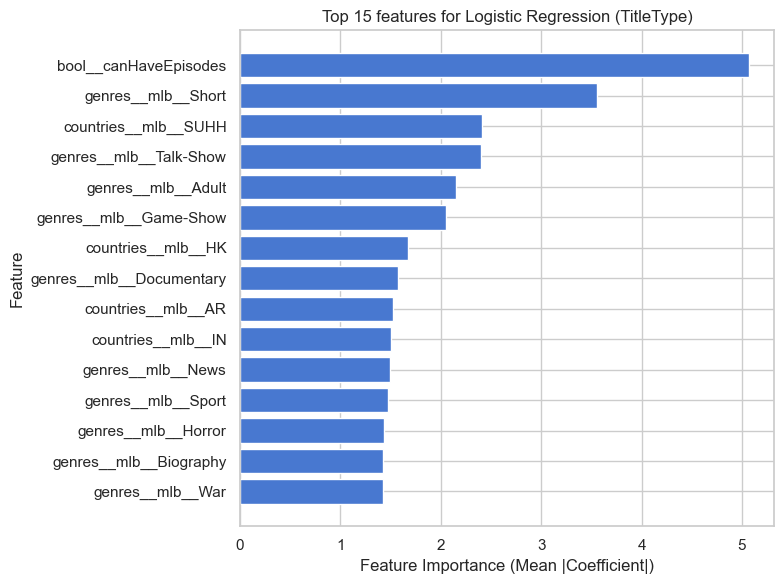
\includegraphics[width=\columnwidth]{../results/images/LR_feat_impo_tt.png}
    \caption{Top 15 most important features for \textit{titleType} (LR).}
    \label{fig:LR_feat_impo_tt.png}
\end{figure}

\subsection{Linear Support Vector Machine}
For Support Vector Machines (SVMs), we scaled numerical features using RobustScaler. We tested the linear kernel and the Radial Basis Function kernel separately to exploit sklearn's optimized LinearSVC implementation.

\subsubsection{Rating}
For LinearSVC, we tested the following parameter grid using a grid search with 5-fold cross validation:

\begin{lstlisting}[basicstyle=\footnotesize\ttfamily,
                   escapeinside={(*@}{@*)}]
  { 'C': [(*@\textbf{0.001}@*), 0.01, 0.1, 1, 10, 100],
    'penalty': ['l1', (*@\textbf{'l2'}@*)],
    'loss': [(*@\textbf{'squared\_hinge'}@*), 'hinge'],
    'max_iter': [5000],
    'class_weight': [None, (*@\textbf{'balanced'}@*)]  }
\end{lstlisting}

It resulted in an average macro F1 of 0.158 for validation and of 0.164 on the training set.

On the test set, w.r.t. Logistic Regression, the model achieved a higher \textbf{macro F1} (\textbf{0.158}), but a lower \textbf{accuracy} (\textbf{0.270}).
Indeed, the F1 for the best performing classes has decreased ((7,8]: 0.496 vs 0.544; (6,7]: 0.215 vs 0.356, (5,6]: 0.259 vs 0.283), in favor of slightly better performances for classes with lower support: the decrease in accuracy is linked to the fact that the model tries to predict these lower support classes more often, rather than focusing merely on the central classes. This led to a notable increase in F1 for (3,4] (0.113 vs 0.04) and (9,10] (0.145 vs 0.046), but it is clear that the model still struggles. The \textbf{PR AUC} is also slightly worse, \textbf{0.175}.

The confusion matrix confirms this tendency: if for Logistic Regression predictions were concentrated on the best performing classes, with many zeros populating the lowest classes, now confusion is spread throughout. 

The most important feature is \textit{tvEpisode} (mean absolute value: 0.175): it is at number one, with negative values, for classes from (2,3] to (5,6] — this would suggest that serialized content is less likely to have bad rating. Classes (7,8] and (8,9] both have \textit{movie} as most important feature, with negative contributions (-0.207 and -190, respectively). This might explain why the latter is mostly classified as the former, which is the class with the highest support.

\subsubsection{Title Type}
The model returned by the grid search yielded an average validation macro F1 of 0.646 (vs 0.654 on the training set); the parameters were \texttt{'C': 0.1, 'class\_weight': 'balanced', 'loss': 'squared\_hinge', 'max\_iter': 5000, 'penalty': 'l1'}.

On the test set, the results were slightly lower than Logistic Regression: \textbf{0.640 macro F1}, \textbf{0.889 accuracy}, \textbf{0.674 PR AUC}. Indeed, performances for almost all classes have decreased to some degree, with a remarkable dip in precision for \textit{videogame} (0.486 vs 0.799).

The overall most important features are the same (\textit{canHaveEpisodes} and genre \textit{Short}), but now only the first stands out (mean absolute value close to 2.5), while \textit{Short} has a similar value to the rest of the top features, < 1.

Unexpectedly, the most important feature for the \textit{titleType} \textit{short} is now \textit{canHaveEpisodes}, with quite an 'advantage' (coef: -2.18, vs genre \textit{Short} 1.43).

\subsection{Support Vector Machine with Radial Basis Function (RBF)}
The power of SVMs comes at a high computational cost, which is why we only tested one kernel function (RBF) and why we opted for an 80/20 holdout, instead of a k-fold cross-validation, to carry out hyperparameter tuning. We also defined a small hyperparameter grid: 
\begin{lstlisting}[basicstyle=\footnotesize\ttfamily,
                   escapeinside={(*@}{@*)}]
  { 'C': [0.1, 1, 10],
    'gamma': ['scale', 0.01, 0.1],
    'class_weight': [None, 'balanced']  }
\end{lstlisting}

\subsubsection{Rating}
The best model returned by the grid search had the following hyperparameters: \texttt{{'C': 10, 'gamma': 0.1, 'class\_weight': None}}. It achieved a macro F1 of 0.265 on the validation set and of 0.698 on the training set, suggesting overfitting.
We therefore reran the grid search, excluding the highest values for C and gamma in order to increase regularization. The best performing model was less overfitted, but also achieved lower results (macro F1 0.206 for validation and 0.316 for training). Its parameters are: \texttt{'C': 1, 'class\_weight': 'balanced', 'gamma': 'scale'}.

On the test set, the overfitted model proved to be the best one, achieving a \textbf{macro F1} of \textbf{0.257} (vs 0.219) and an \textbf{accuracy} of \textbf{0.431} (vs 0.314). The resulting \textbf{PR AUC }is \textbf{0.231}. This model is also the best performing one thus far, with improvements observed across almost all classes.

Looking at the confusion matrix, we can see that the model doesn't completely snub lower support classes, like Logistic Regression did, but is more accurate than LinearSVC. Especially for the more popular (and better performing) classes, confusion is mostly among neighboring classes.

\subsubsection{Title Type}
Similarly to what had happened with \textit{rating}, the first grid search returned an overfitted model (macro F1 for validation: 0.746, vs for training: 0.905). Forcing regularization resulted in less overfitting, but also in a much poorer performance (validation macro F1: 0.206, train macro F1: 0.316); for this reason, we chose the first classifier. Its parameters are: \texttt{'C': 10, 'class\_weight': None, 'gamma': 'scale'}.

On the test set, this model clears all previous attempts, with a \textbf{macro F1} of \textbf{0.746} and an \textbf{accuracy} of \textbf{0.938}.

The performances for all classes increased. \textit{tvEpisode} now achieves an F1 of 0.99; \textit{videogame} improved greatly, reaching 0.884 F1. Nevertheless, we only get a \textbf{PR AUC} of \textbf{0.689}; indeed, the curves in Fig. \ref{fig:pr_svm_rbf_tt.png} show how the precision for half of the classes sinks at around 60\% recall. This means that while the model shows excellent performance metrics on a per-class basis, it has difficulty maintaining a reliable performance when attempting to comprehensively identify instances of minority classes.

\begin{figure}
    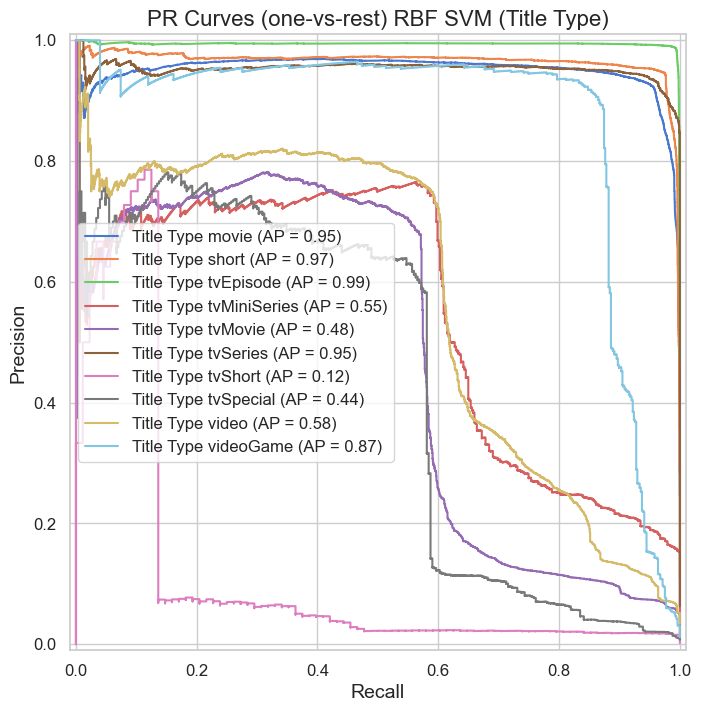
\includegraphics[width=\columnwidth]{../results/images/pr_svm_rbf_tt.png}
    \caption{PR curves for \textit{titleType} (SVM with RBF).}
    \label{fig:pr_svm_rbf_tt.png}
\end{figure}

\subsection{Random Forest}
Since this method is based on trees, no scaling is needed for numerical features. To cut computational costs, we used 3-fold cross validation during hyperparameter tuning.

Indeed, there are many possible hyperparameters to tune. For each task, we ran three Randomized Searches, for a varying number of estimators — 100, 300 and 500, respectively. For each, we tested the same 100 random combinations of parameters from the following grid:
\begin{lstlisting}[basicstyle=\footnotesize\ttfamily,
                   escapeinside={(*@}{@*)}]
  { 'criterion': ["gini", "entropy"],
    'max_depth': [None, 5, 15, 25],
    'min_samples_split': [2, 5, 10],
    'min_samples_leaf': [1, 5, 10],
    'class_weight': [None, 'balanced']  }
\end{lstlisting}

\subsubsection{Rating}
Before proceeding with hyperparameter tuning, we first tested a Random Forest using default parameters, which yielded an average validation macro F1 of 0.296, and an even better 0.302 macro F1 score on the test set.

As shown in Fig. \ref{fig:rf_comparison_n_estimators_rating.png}, the number of estimators is not a strong driver of performance. Although the performance of the other two models was very close, we chose the best model with 300 base classifiers, which yielded an average macro F1 equal to 0.308 for validation, and equal to 0.968 for train. Its parameters are: \texttt{{'n\_estimators': 300, 'min\_samples\_split': 5, 'min\_samples\_leaf': 1, 'max\_depth': None, 'criterion': 'gini', 'class\_weight': 'balanced'}}.

\begin{figure}
    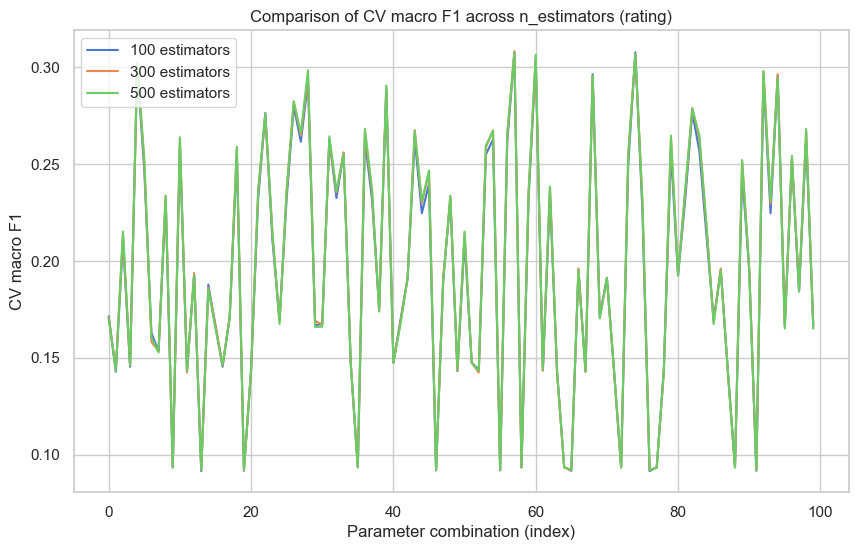
\includegraphics[width=\columnwidth]{../results/images/rf_comparison_n_estimators_rating.png}
    \caption{Avg cross-validation macro F1 for different parameter configurations across varying numbers of estimators for \textit{rating} (RF).}
    \label{fig:rf_comparison_n_estimators_rating.png}
\end{figure}


Whether such a gap between validation and train macro F1 should be seen as a sign of overfitting for Random Forest is debated in the literature: it has been argued that, even if the single trees can overfit, they tend to do so in different ways, and that combining them in an ensemble reduces the overall variance. Thus, although pruning the individual trees can be beneficial, unless the dataset is very simple, we could consider Random Forest as particularly robust against overfitting.

The model's performance on the test set increases, making it the best model thus far: it achieves a \textbf{macro F1} of \textbf{0.325}, an \textbf{accuracy} of \textbf{0.452}, and a \textbf{PR AUC} of \textbf{0.318}.

It achieves the most balanced performance, with six classes out of ten scoring an F1 >= 0.3. Confusion remains spread out for the minority classes (from 0 to 4), whereas for the others it remains concentrated amongst neighboring classes.

The Mean Decrease in Impurity (MDI) returned as the most important features \textit{numVotes} and startYear (almost 0.10), followed by \textit{totalCredits} (around 0.9).

\subsubsection{Title Type}
The default model achieved an average macro F1 of 0.707 on validation and a score of 0.728 on the test set.

The performances for the different parameters combinations tested during the Random Searches were again very similar, with the configurations using 100 estimators yielding marginally lower scores. Indeed, the three best models shared the same hyperparameter values. We chose the configuration with 300 trees: the validation performances were only marginally better than that of the 500-trees model, but we also favored simplicity.

The model yielded 0.767 and 0.975 for validation and training, respectively. Its hyperparameter configuration is the following: \texttt{'n\_estimators': 300, 'min\_samples\_split': 10, 'min\_samples\_leaf': 1, 'max\_depth': None, 'criterion': 'entropy', 'class\_weight': 'balanced'}. 

On the test set, it clears previous models, achieving \textbf{0.777 macro F1} and \textbf{0.940 accuracy}. Half of the classes yield F1 > 0.95. It generalizes better on the minority classes \textit{tvMovie} and \textit{tvMiniSeries}: although there is still confusion with the more popular \textit{movie} and \textit{tvSeries}, they are correctly classified most of the time (cf. the confusion matrix in Fig. \ref{fig:rf_conf_matrix_tt.png}).

This model's superiority across decision thresholds is supported by the PR curves in Fig. \ref{fig:rf_pr_curves.png}, and further quantified by its \textbf{PR AUC} of \textbf{0.818}.

\begin{figure}
    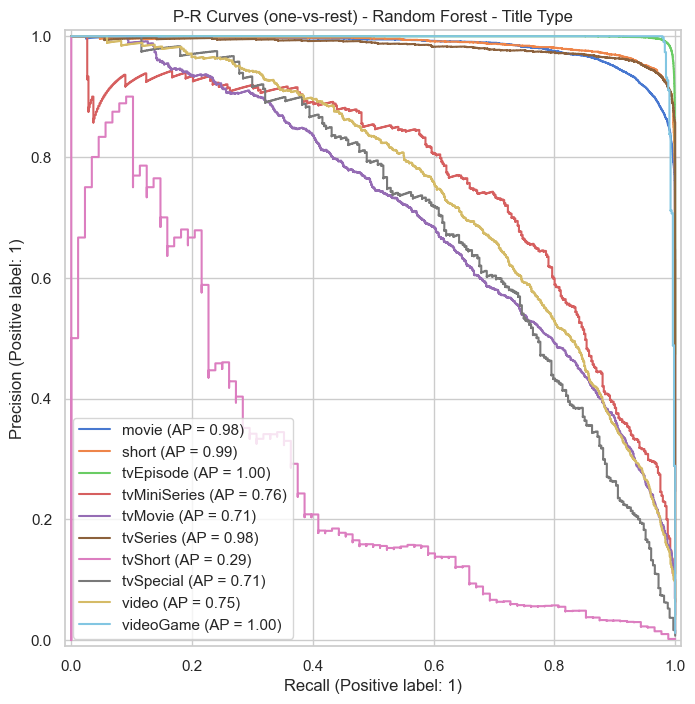
\includegraphics[width=\columnwidth]{../results/images/rf_pr_curves.png}
    \caption{PR curves for \textit{titleType} (RF).}
    \label{fig:rf_pr_curves.png}
\end{figure}

\begin{figure}
    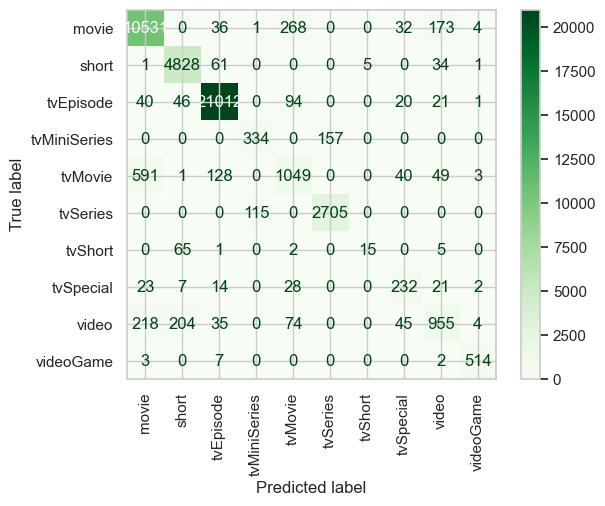
\includegraphics[width=\columnwidth]{../results/images/rf_conf_matrix_tt.png}
    \caption{Confusion matrix for \textit{titleType} (RF).}
    \label{fig:rf_conf_matrix_tt.png}
\end{figure}

Checking the 15 most important features (Fig \ref{fig:rf_feat_impo_tt.png}), we see how the two most important features for the Logistic Regression model, \textit{canHaveEpisodes} and the genre \textit{Short}, have been overtaken by \textit{runtimeMinutes}. Indeed, we had uncovered a relationship between \textit{runtimeMinutes} and \textit{titleType} in Subsec. \ref{handling_nan}.

\begin{figure}
    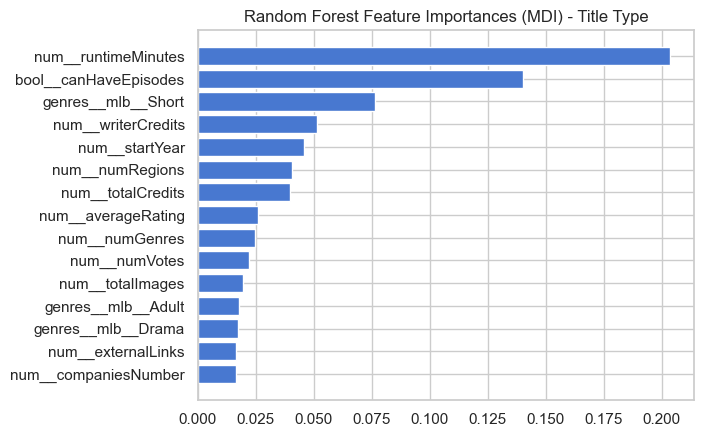
\includegraphics[width=\columnwidth]{../results/images/rf_feat_impo_tt.png}
    \caption{Top 15 most important features for \textit{titleType} (RF).}
    \label{fig:rf_feat_impo_tt.png}
\end{figure}

Finally, it's worth pointing out that prior experimentation keeping the default hyperparameter \texttt{'class\_weight': None} instead of \texttt{'balanced'} lead to a best model scoring a significantly lower macro F1 score of 0.728. This is indicative of the importance of this hyperparameter for this unbalanced task.

\subsection{LightGBM}


\subsection{Multilayer Perceptron}


\subsection{Conclusions}
\section{Explainability: SHAP for Random Forest Classification}
\section{Advanced Regression}
In this section, we will discuss the performance of two advanced regression methods in predicting the \textit{averageRating}.

We used the same preprocessing pipeline detailed in Subsec. \ref{classification_preprocessing} and the feature set we had used for the Multilayer Perceptron.

We evaluated performances using the Determination Coefficient (R2) and the Mean Squared Error (MSE). To set a baseline, we used a DummyRegressor which always predicts the mean of the target values observed in the training set, which yielded a \textbf{R2} of \textbf{0} and a \textbf{MSE} of \textbf{1.819} (equal to the variance of the target variable).

\subsection{Random Forest Regressor}

\subsection{XGBoost Regressor}


\section{Time Series Analysis}
\label{time_series_analysis}
\subsection{Data Understanding and Preparation}\label{sec:ts_preparation}
This dataset contains data on the domestic (US and Canada) daily gross income at the box office for 1,134 movies, measured from their release date up to 100 days after release.
The dataset was extracted from Box Office Mojo\footnote{\url{https://www.boxofficemojo.com/}} and contains no missing values, because shorter time series were padded using noise augmented mean.
Each time series was associated with the movie IMDB id, genre and rating (both continuous average rating and a binned version).
In addition to the provided data, we used the IMDB free api\footnote{\url{https://imdbapi.dev/}} to retrieve some additional information about the titles represented in the dataset: title and release year of the movie, runtime (in minutes) number of votes, countries of origin, number of awards and nominations.
We additionally aggregated the box office data as a rough estimate of the total gross income of the movie.

We then splitted our initial dataset reserving 25\% of records for testing and conducted the rest of our analysis exclusively on the training set, as to prevent data leakage.

\subsubsection{Univariate analysis of variables}
The distribution of number of votes, awards, nominations and total gross income show all a pronounced right skew, which is not unexpected. 90\% of records had received awards of nominations.
All records display normal runtimes for movies (between 90 and 200 minutes), except for 3 documentaries which were shorter than 45 minutes.
We were able to detect some outliers also w.r.t. the release year: only two titles were released before 2010 (one in 1969 and one in 1984).

As for the distribution with respect to genres, any given movie can have more than one genre and the most popular genre was \emph{Drama} (48\%), followed by \emph{Comedy} (36\%), \emph{Action} and \emph{Adventure} (each of these 32\%).

We also inspected the distribution of the binned version of rating, finding a considerable unbalance among classes, with \emph{Medium} and \emph{High} being the most frequent ones and the \emph{Low} class representing less than 1\% of titles (cf Fig. \ref{fig:ts_rating_distribution}).

\begin{figure}
    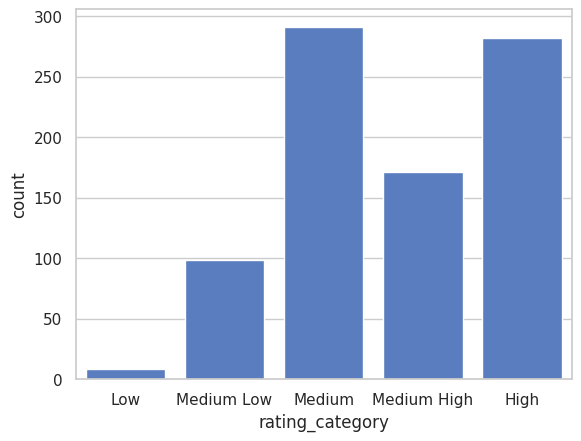
\includegraphics[width=\columnwidth]{../results/images/ts_rating_distribution.png}
    \caption{Distribution of rating category in the Time Series dataset.}\label{fig:ts_rating_distribution}
\end{figure}

\subsubsection{Multivariate analysis of variables}
\begin{figure}[t]
    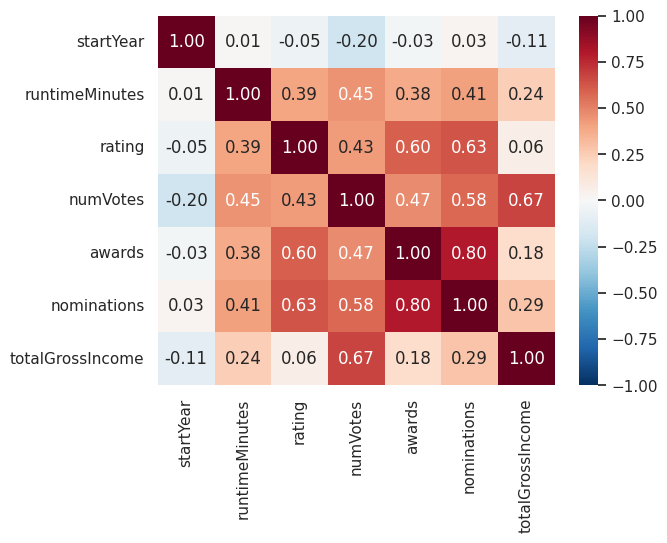
\includegraphics[width=\columnwidth]{../results/images/ts_feat_correlation.png}
    \caption{Correlation of numeric features.}\label{fig:ts_feat_correlation}
\end{figure}

Figure \ref{fig:ts_feat_correlation} reports the Spearman correlation coefficient for pairs of numeric features.
Besides obviously being correlated with each other, both awards and nominations are positively correlated with both the number of votes and rating.
We also observe a moderate to strong positive correlation between the estimated gross income and number of votes.
Perhaps surprisingly, total gross income is only weakly correlated with rating.

Positive correlation of the number votes with rating is something we didn't observe in the IMDB dataset, were, on the contrary these two features were weakly negatively correlated.
We think this may be due to the fact that movies have on average lower ratings than TV Episodes, which, in turn, have fewer votes than movies.
Since the current dataset is limited to movies, we do not observe this (spurious) relationship anymore.

\subsubsection{Visualization}

\begin{figure}
    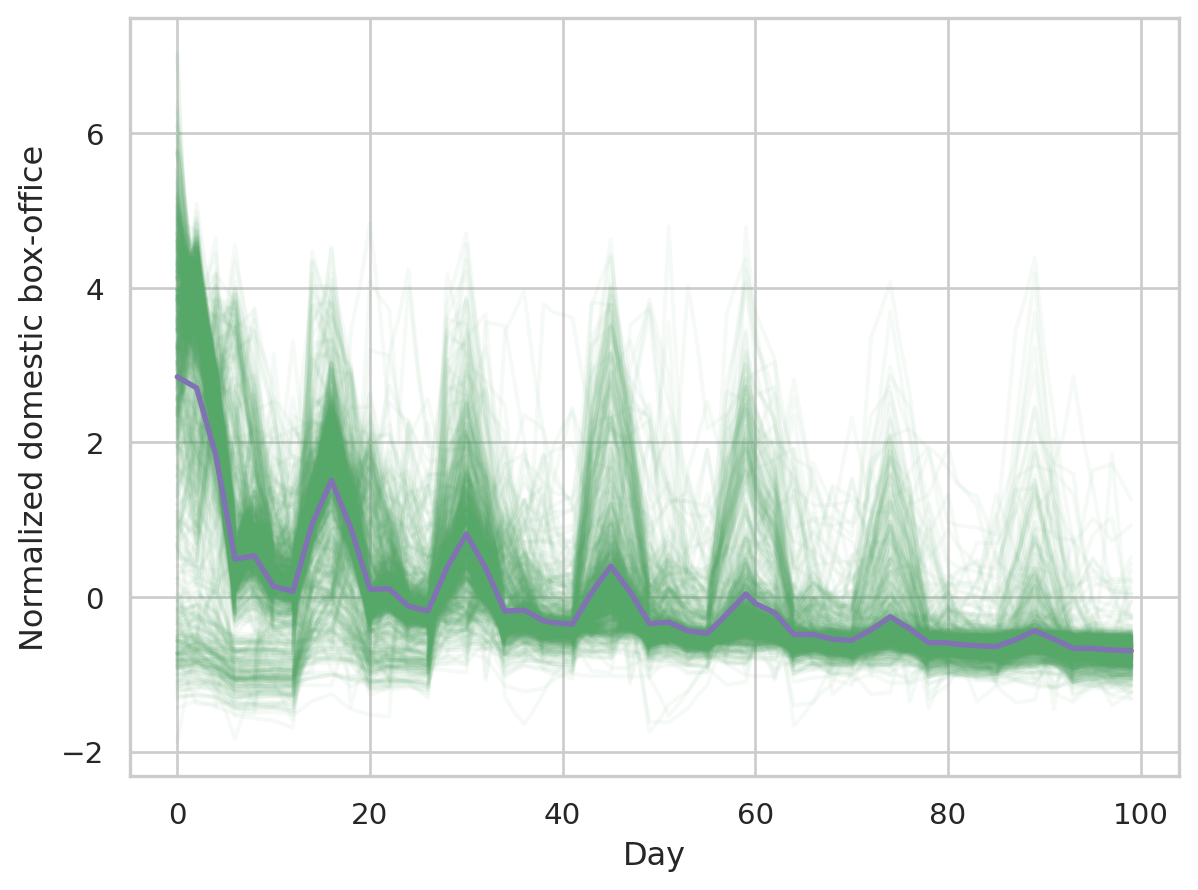
\includegraphics [width=\columnwidth]{../results/images/ts_understanding_viz.png}
    \caption{Time series (and mean time series, in purple) after amplitude scaling}\label{fig:ts_understanding_viz}
\end{figure}

We conclude our understanding visualizing the signals for all time series after amplitude scaling (fig. \ref{fig:ts_understanding_viz}).
Even from this simple visualization we are able to draw some interesting insights.

First of all our time series in general show slightly negative trend and some seasonality with a cycle over around 14 timestamps: this observation was confirmed when we extracted Catch22 features from the time series and were able to verify that most of them had a periodicity of 13 or 14.
This finding, which we initially took at face value, was somewhat puzzling, because we expected a day of week seasonality, with peaks in the weekends, while it made no sense for peaks to occur every other week.
Surely enough, when we finally checked against the original data on Box Office Mojo, we were able to confirm that the observed peaks are, in fact, the effect of day of week seasonality, and that the time series were altered before we received them, either during the extraction or during the preprocessing.

In addition to this discovery, we also were able to observe that, while most movies have profits well over the mean in the first several days after release, some others got a slow start at the box office.
We were able to identify 145 movies that performed below average in the first day of box office. While this is a very coarse distinction, which incurs in some false positives, it was later confirmed by clustering.
In addition to lower box office profits in the first days after release, these `late bloomers' show no clear linear trend (in opposition to the negative trend observed for other movies) and tend to peak on the third weekend after release. We also observed that these were not, for the most part (93\%), action movies.
\subsection{Clustering}\label{sec:ts_clustering}
In our clustering analysis of time series we adopted two different approaches to the measure of similarity: shape-based similarity and structural similarity.

For the shape-based approach, we first subjected the time series to amplitude scaling and then measured the distances between records employing DTW as to minimize the impact of misaligned time series.
Since our time series were very short, we didn't deem it necessary to apply any approximation method to the original signal; we did, however impose constraints (Sakoe-Chiba Band with radius 0.1) on the warping in order to reduce computation time and avoid pathological warpings.

For the global structural approach, we extracted mean, standard deviation and Catch22 features from the raw signals (without amplitude scaling) and then computed Euclidean Distance on this new feature matrix (which was normalized using a Standard Scaler).

\subsubsection{Shape-based clustering}

\begin{figure}
    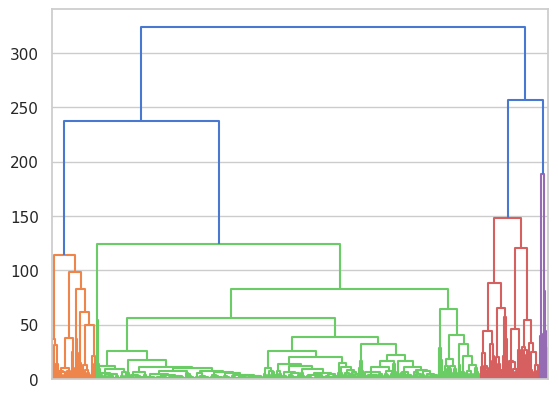
\includegraphics[width=\columnwidth]{../results/images/tsclust_hierarhical_dendrogram.png}
    \caption{Dendrogram for shape-based hierarhical clustering.}\label{fig:tsclust_dendrogram}
\end{figure}

\begin{figure}
    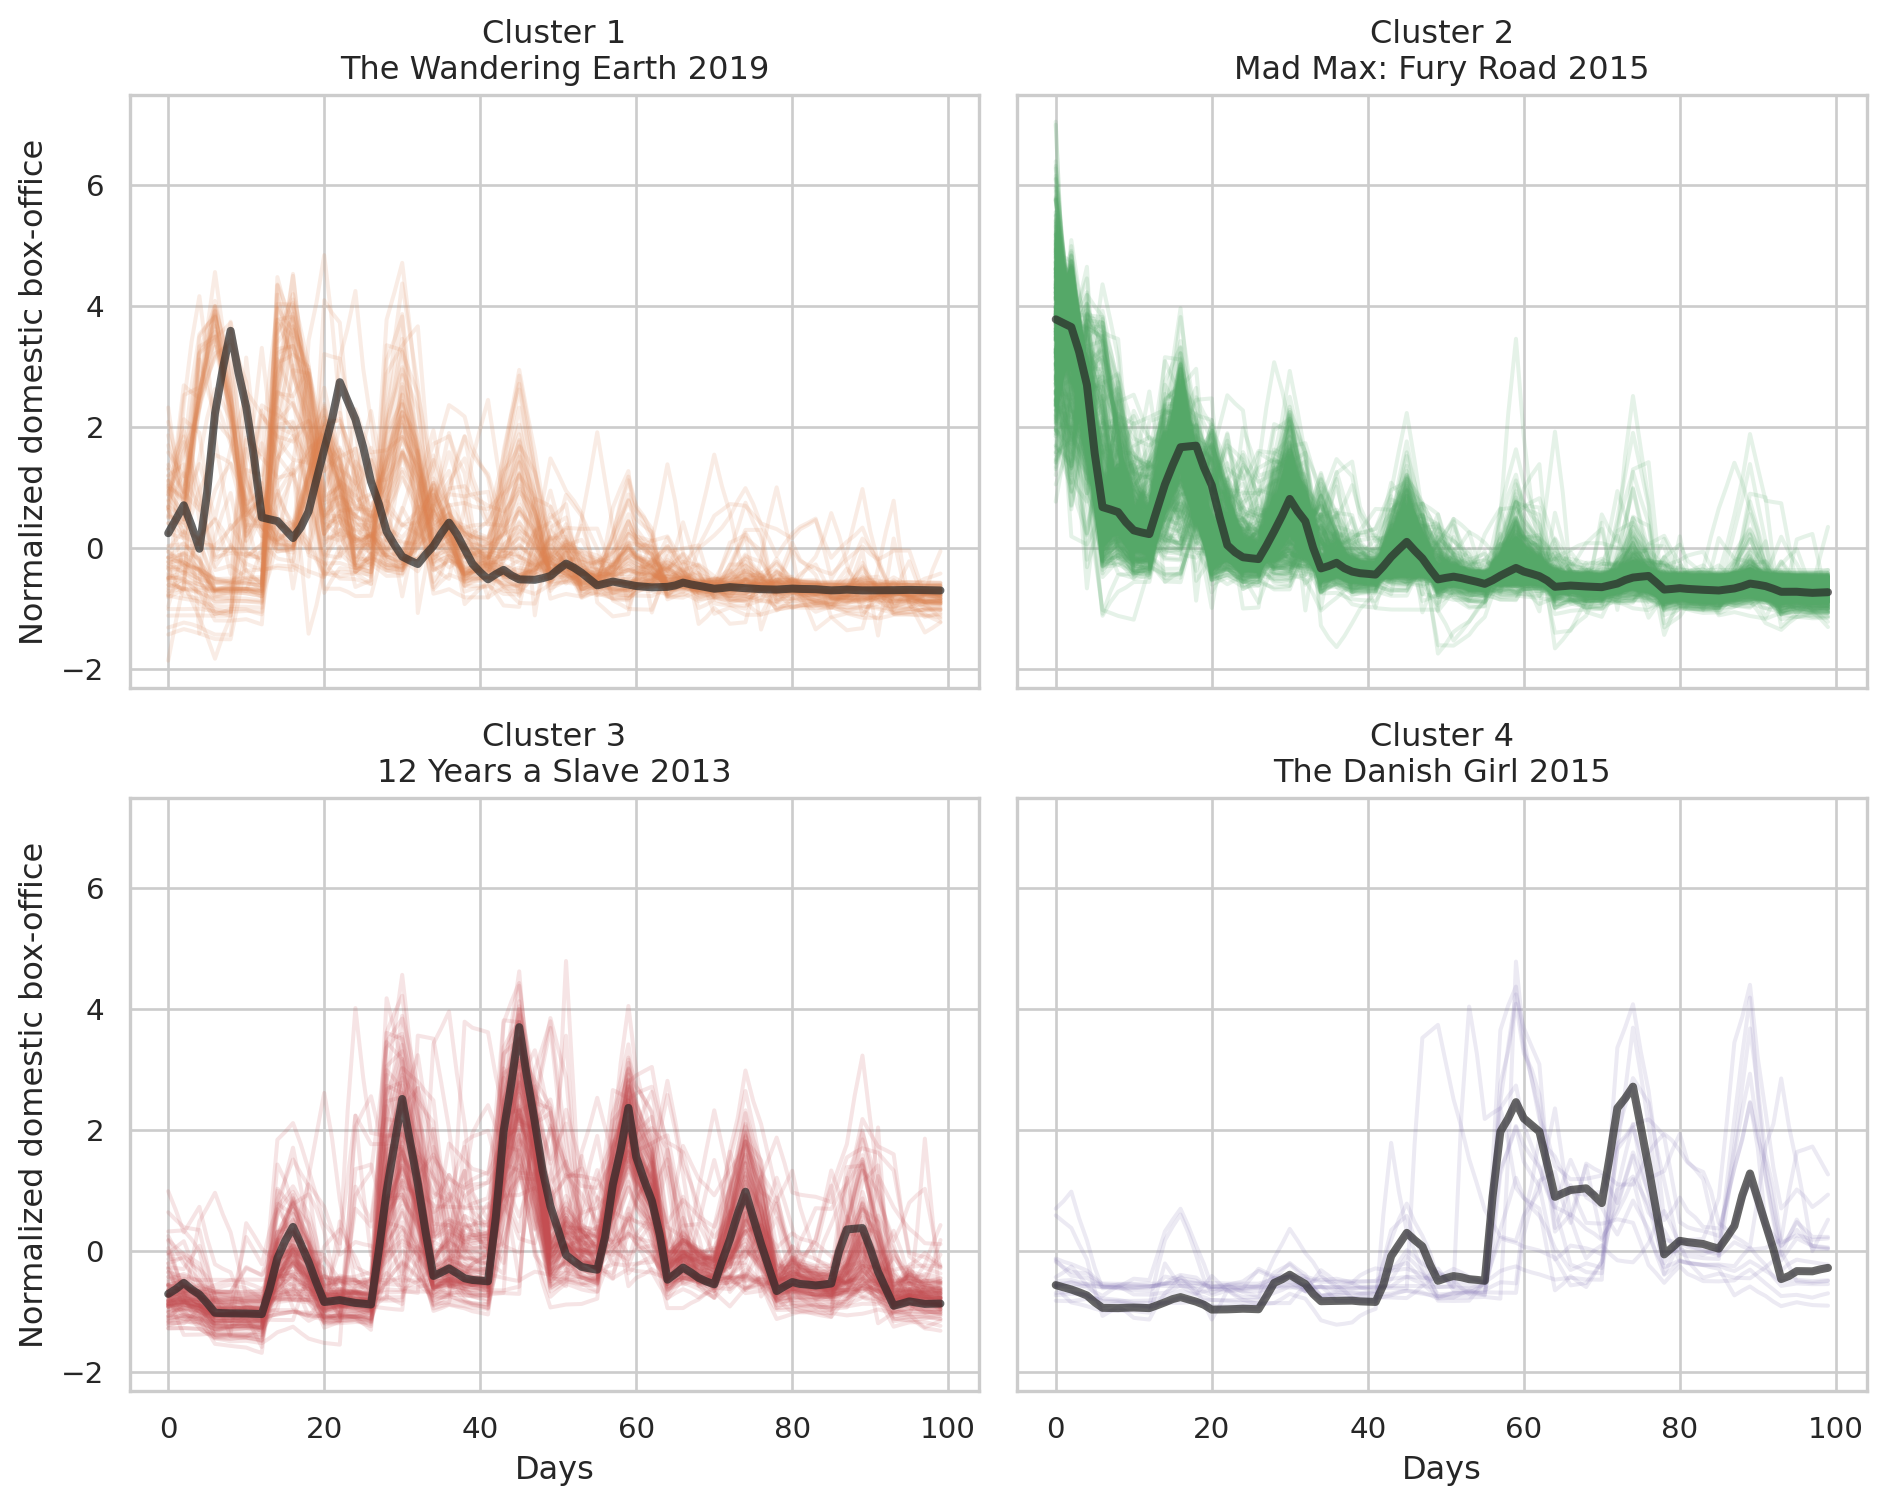
\includegraphics[width=\columnwidth]{../results/images/tsclust_hierarhical_series.png}
    \caption{Clusters obtained by hierarchical clustering and respective cluster medoids (in black).}\label{fig:tsclust_hierarchical_series}
\end{figure}

\begin{figure}
    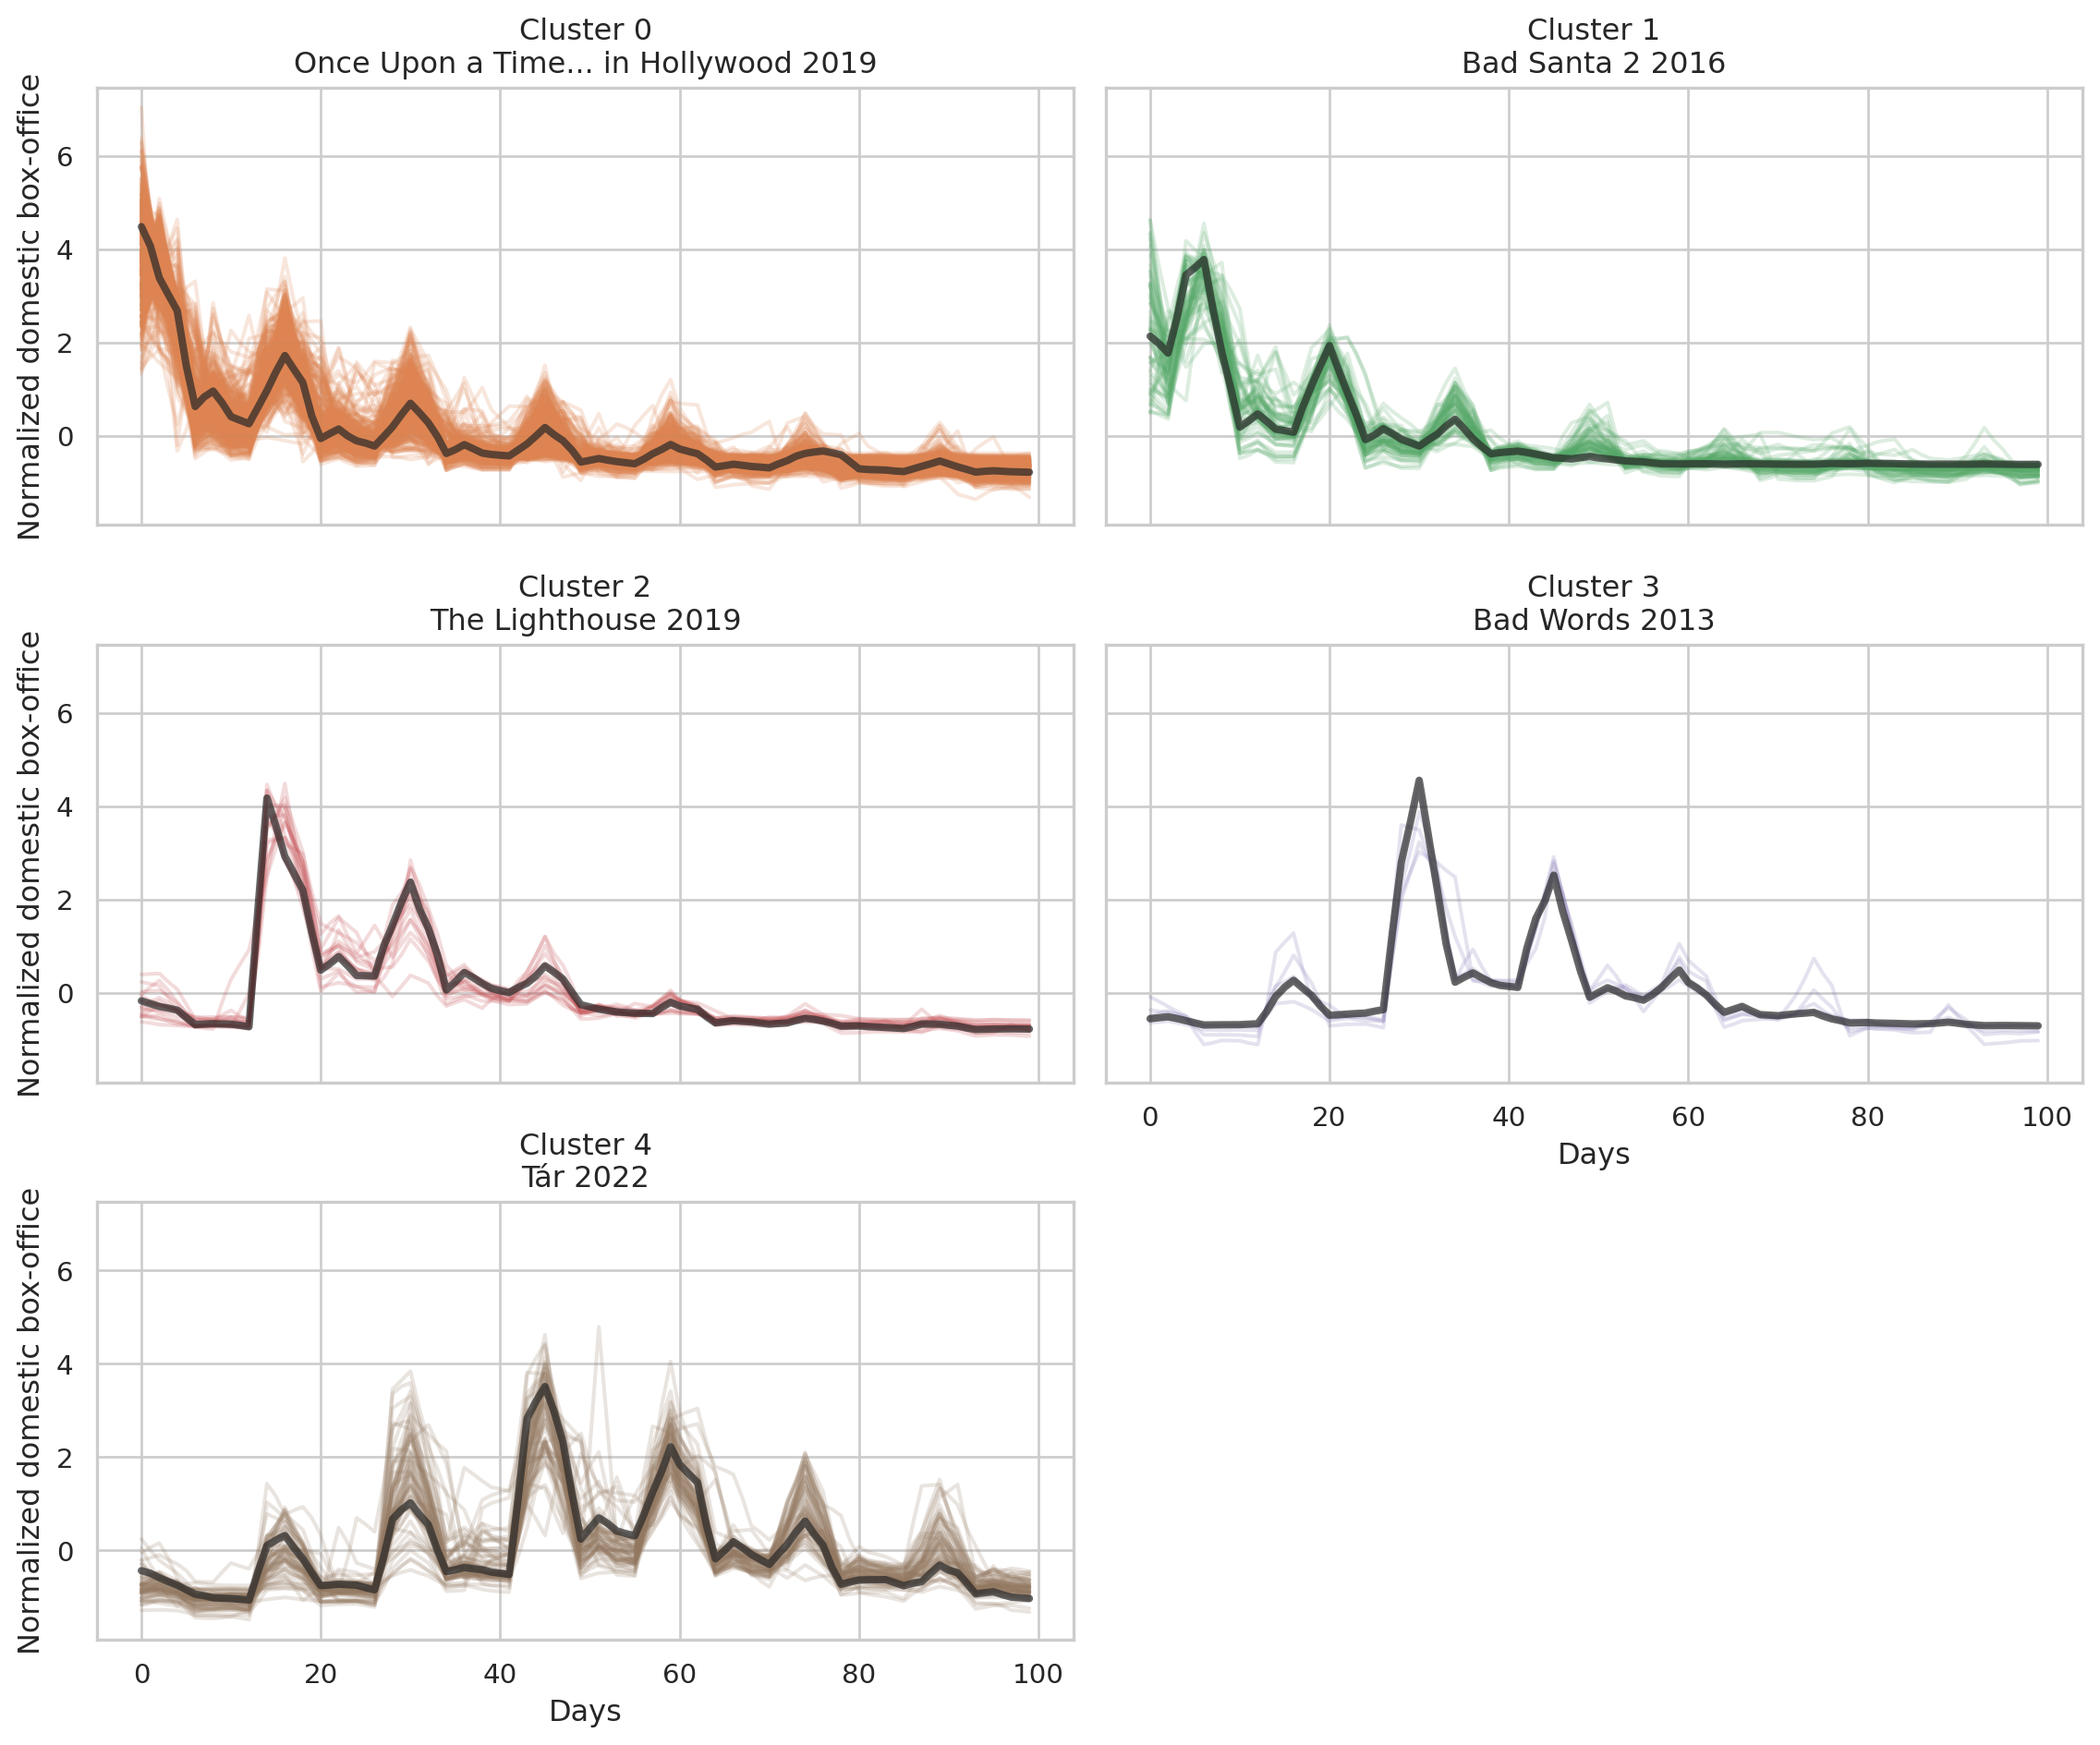
\includegraphics[width=\columnwidth]{../results/images/tsclust_density_series.png}
    \caption{Clusters obtained by density-based clustering and respective cluster medoids (in black).}\label{fig:tsclust_density_series}
\end{figure}

Since in our understanding phase we were able to recognize two distinct patterns, we first of all run K-Means with k=2 and obtained results very similar to those previously discussed. This clustering obtained a silhouette score of 0.85 and was able to identify 159 `late bloomers'.

We then experimented with different linkage criteria for hierarchical clustering, selecting in the end average linkage, which yielded the best dendrogram (Fig. \ref{fig:tsclust_dendrogram}).
After selecting an appropriate threshold, we obtained 4 clusters of very different sizes (C1: 75, C2: 658, C3: 101, C4:15). This clustering obtained a silhouette score of 0.77.

Signals for clustered time series and cluster medoids are visualized in Fig. \ref{fig:tsclust_hierarchical_series}: it can be easily seen that, while C2 and C3 can be identified respectively with instant hits and `late bloomers', the identity of movies from C1 and C4 is more confused.
Detailed analysis of silhouette scores revealed that many records from C4 and especially C1 have negative silhouette scores, suggesting that they were assigned to the wrong cluster.

We then run Principal Component Analysis on the dataset and visualized clusters on the two first components, which together explain more than 60\% of variance (Fig. \ref{fig:hier_pca}, cluster medoids are showed in black).

Inspecting the PCA Eigenvectors, we found out that the first component is mainly concerned with timestamps from the first week or so, which explains why records from C2 (and some records from C1) have positive values in this component, while the `late bloomers' from C3 have very negative values.
Also, observing the distribution of records from C1 along the first component, it is clear why more than half of them have a negative silhouette score, since they clearly should belong to C2.
In contrast, K-Means, clearly separates the two clusters along the first component.

\begin{figure*}[t]
    \centering
    \begin{subfigure}{0.45\textwidth}
        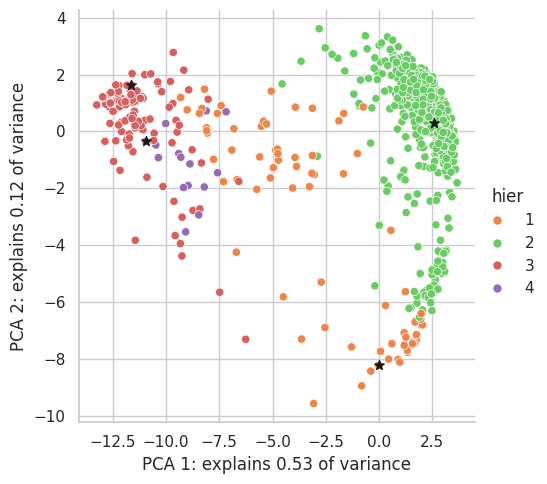
\includegraphics[width=\textwidth]{../results/images/tsclust_hier_pca.png}
        \caption{Hierachical clustering PCA.}\label{fig:hier_pca}
    \end{subfigure}
    \begin{subfigure}{0.45\textwidth}
        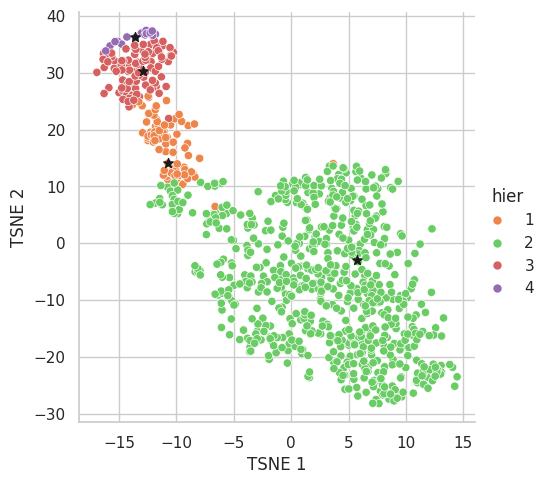
\includegraphics[width=\textwidth]{../results/images/tsclust_hier_tsne.png}
        \caption{Hierarchical clustering tSNE.}
    \end{subfigure}
    \begin{subfigure}{0.45\textwidth}
        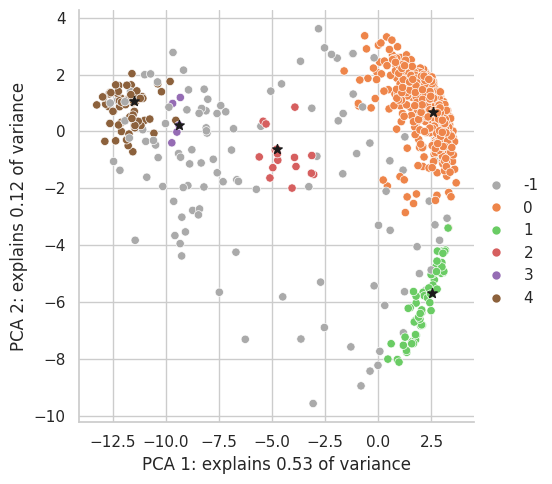
\includegraphics[width=\textwidth]{../results/images/tsclust_density_pca.png}
        \caption{DBSCAN clustering PCA.}\label{fig:density_pca}
    \end{subfigure}
    \begin{subfigure}{0.45\textwidth}
        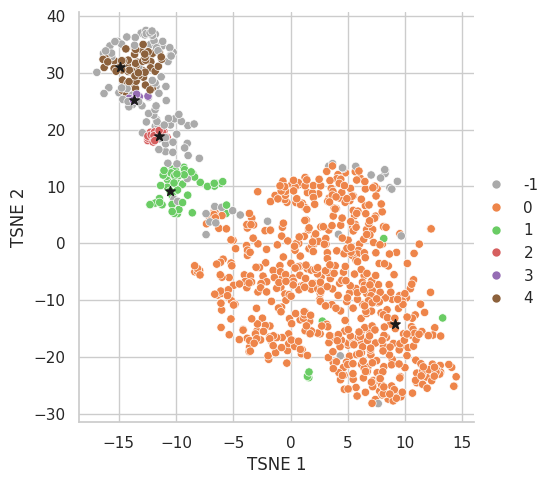
\includegraphics[width=\textwidth]{../results/images/tsclust_density_tsne.png}
        \caption{DBSCAN clustering tSNE.}
    \end{subfigure}
    \caption{Clusters and cluster medoids for hierarchical clustering and DBSCAN visualized with two dimensionality reduction techniques.}\label{fig:clusters}
\end{figure*}

We also visualized the clusters using tSNE on the DTW distance matrix.
We choose this projection for its ability of preserving the local structure of the dataset.
While tSNE was able to convey some information on the numeric relative dimensions of different clusters, and was able to visualize clusters nicely, in the end it proved less interesting, because of its inability of revealing the global structure of the dataset and of conveying the variable density of our clusters.

Inspection of the PCA visualization convinced us that extraction of clusters with a density-based method was viable.
Since a series of run with different radii failed to return any interesting clusters, we decided to pursue a different approach: we run OPTICS (with \texttt{minPts=4}) to completion on a reduced version of the dataset, using the first 5 components created by PCA (which capture more than 80\% of variance). We then visualized the reachability plot and choose an appropriate radius with which to run DBSCAN using the reachability distances computed by OPTICS.
DBSCAN detected 116 noise points and returned five clusters of varying sizes (C0: 594, C1:57, C2: 16, C3: 5 and C4: 62, see Fig. \ref{fig:tsclust_density_series}).

We computed the silhouette score for non noise points on the DTW distance matrix, in order to have results comparable with the other clustering methods.
We found that, while globally the silhouette was a little worse than for the previous methods (0.69), essentially no record showed signs of being misclassified.

Inspection of the PCA visualization (Fig. \ref{fig:density_pca}) shows that this method doesn't fall into the pitfalls of the hierarchical clustering, for example finding a good separation between C0 and C1.

However, while C0 and C1 are fully satisfactory, respectively clustering together instant hits and movies with a similar pattern to instant hits, but with a less explosive first weekend, it looks to us that the clustering of records with lower values on the first PCA component is more contentious because of DBSCAN's inability to detect clusters of different densities.
Arguably the `late bloomers' from C3 and C4 should be clustered together (probably with some noise points).
C2, despite its size, captured our interest, because it was able to detect a pattern no other clustering method was able to capture. It seems to us that movies in this cluster have a slow start at the box office, but, differently from our `late bloomers', they explode on the first weekend after the release and then display a behavior very similar to instant hits.
We hypothesized that this cluster was grouping together movies that were pre-released in a limited fashion.

\subsubsection{Distribution of shape-based clusters w.r.t. exogenous features}
\begin{figure}
    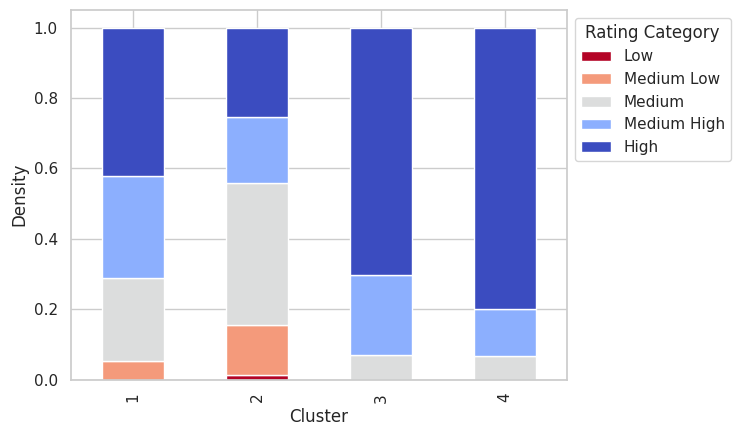
\includegraphics[width=\columnwidth]{../results/images/dist_clust_rating_cat.png}
    \caption{Distribution of binned rating by cluster (hierarchical).}
\end{figure}

In this analysis we concentrated our attention on instant hits from C3 and `late bloomers' from C2 returned by the hierarchical clustering.
We noticed that `late bloomers' have on average a lower average box office (median in the 100k) than instant hits (median in the millions).
This is a valuable finding, since we applied amplitude scaling on the time series before analysis.

In addition to that, we found that `late bloomers' are treated more favorably in terms of rating, as can be seen from  and receive on average more awards and nominations.
Action movies are severely underrepresented among `late bloomers' (only 5\% vs 38\% of records from C2 and 32\% globally), while dramatic movies are overrepresented, since, despite making up about half of the dataset, they make up more than 85\% of C3.

\subsubsection{Global structural features clustering}\label{sec:tsclust_features}
We ran hierarchical clustering on time series structural features experimenting with different linkage criteria and selecting the one that gave use the best dendrogram (Ward).
We obtained four clusters and a mean silhouette of 0.21 (it should be noted that we do not invite comparison with the silhouette obtained by shape-based methods, since this clustering was performed on an entirely different distance matrix).

From Fig. \ref{fig:tsclust_structure.png} we can see that also this clustering method was able to detect the patterns observed previously, albeit in a less marked way. C1 and C2 (which are later merged in a single cluster) are mainly made up of `late bloomers', while C3 and C4 group together instant hits (C3 and C4 are sisters).

\begin{figure}
    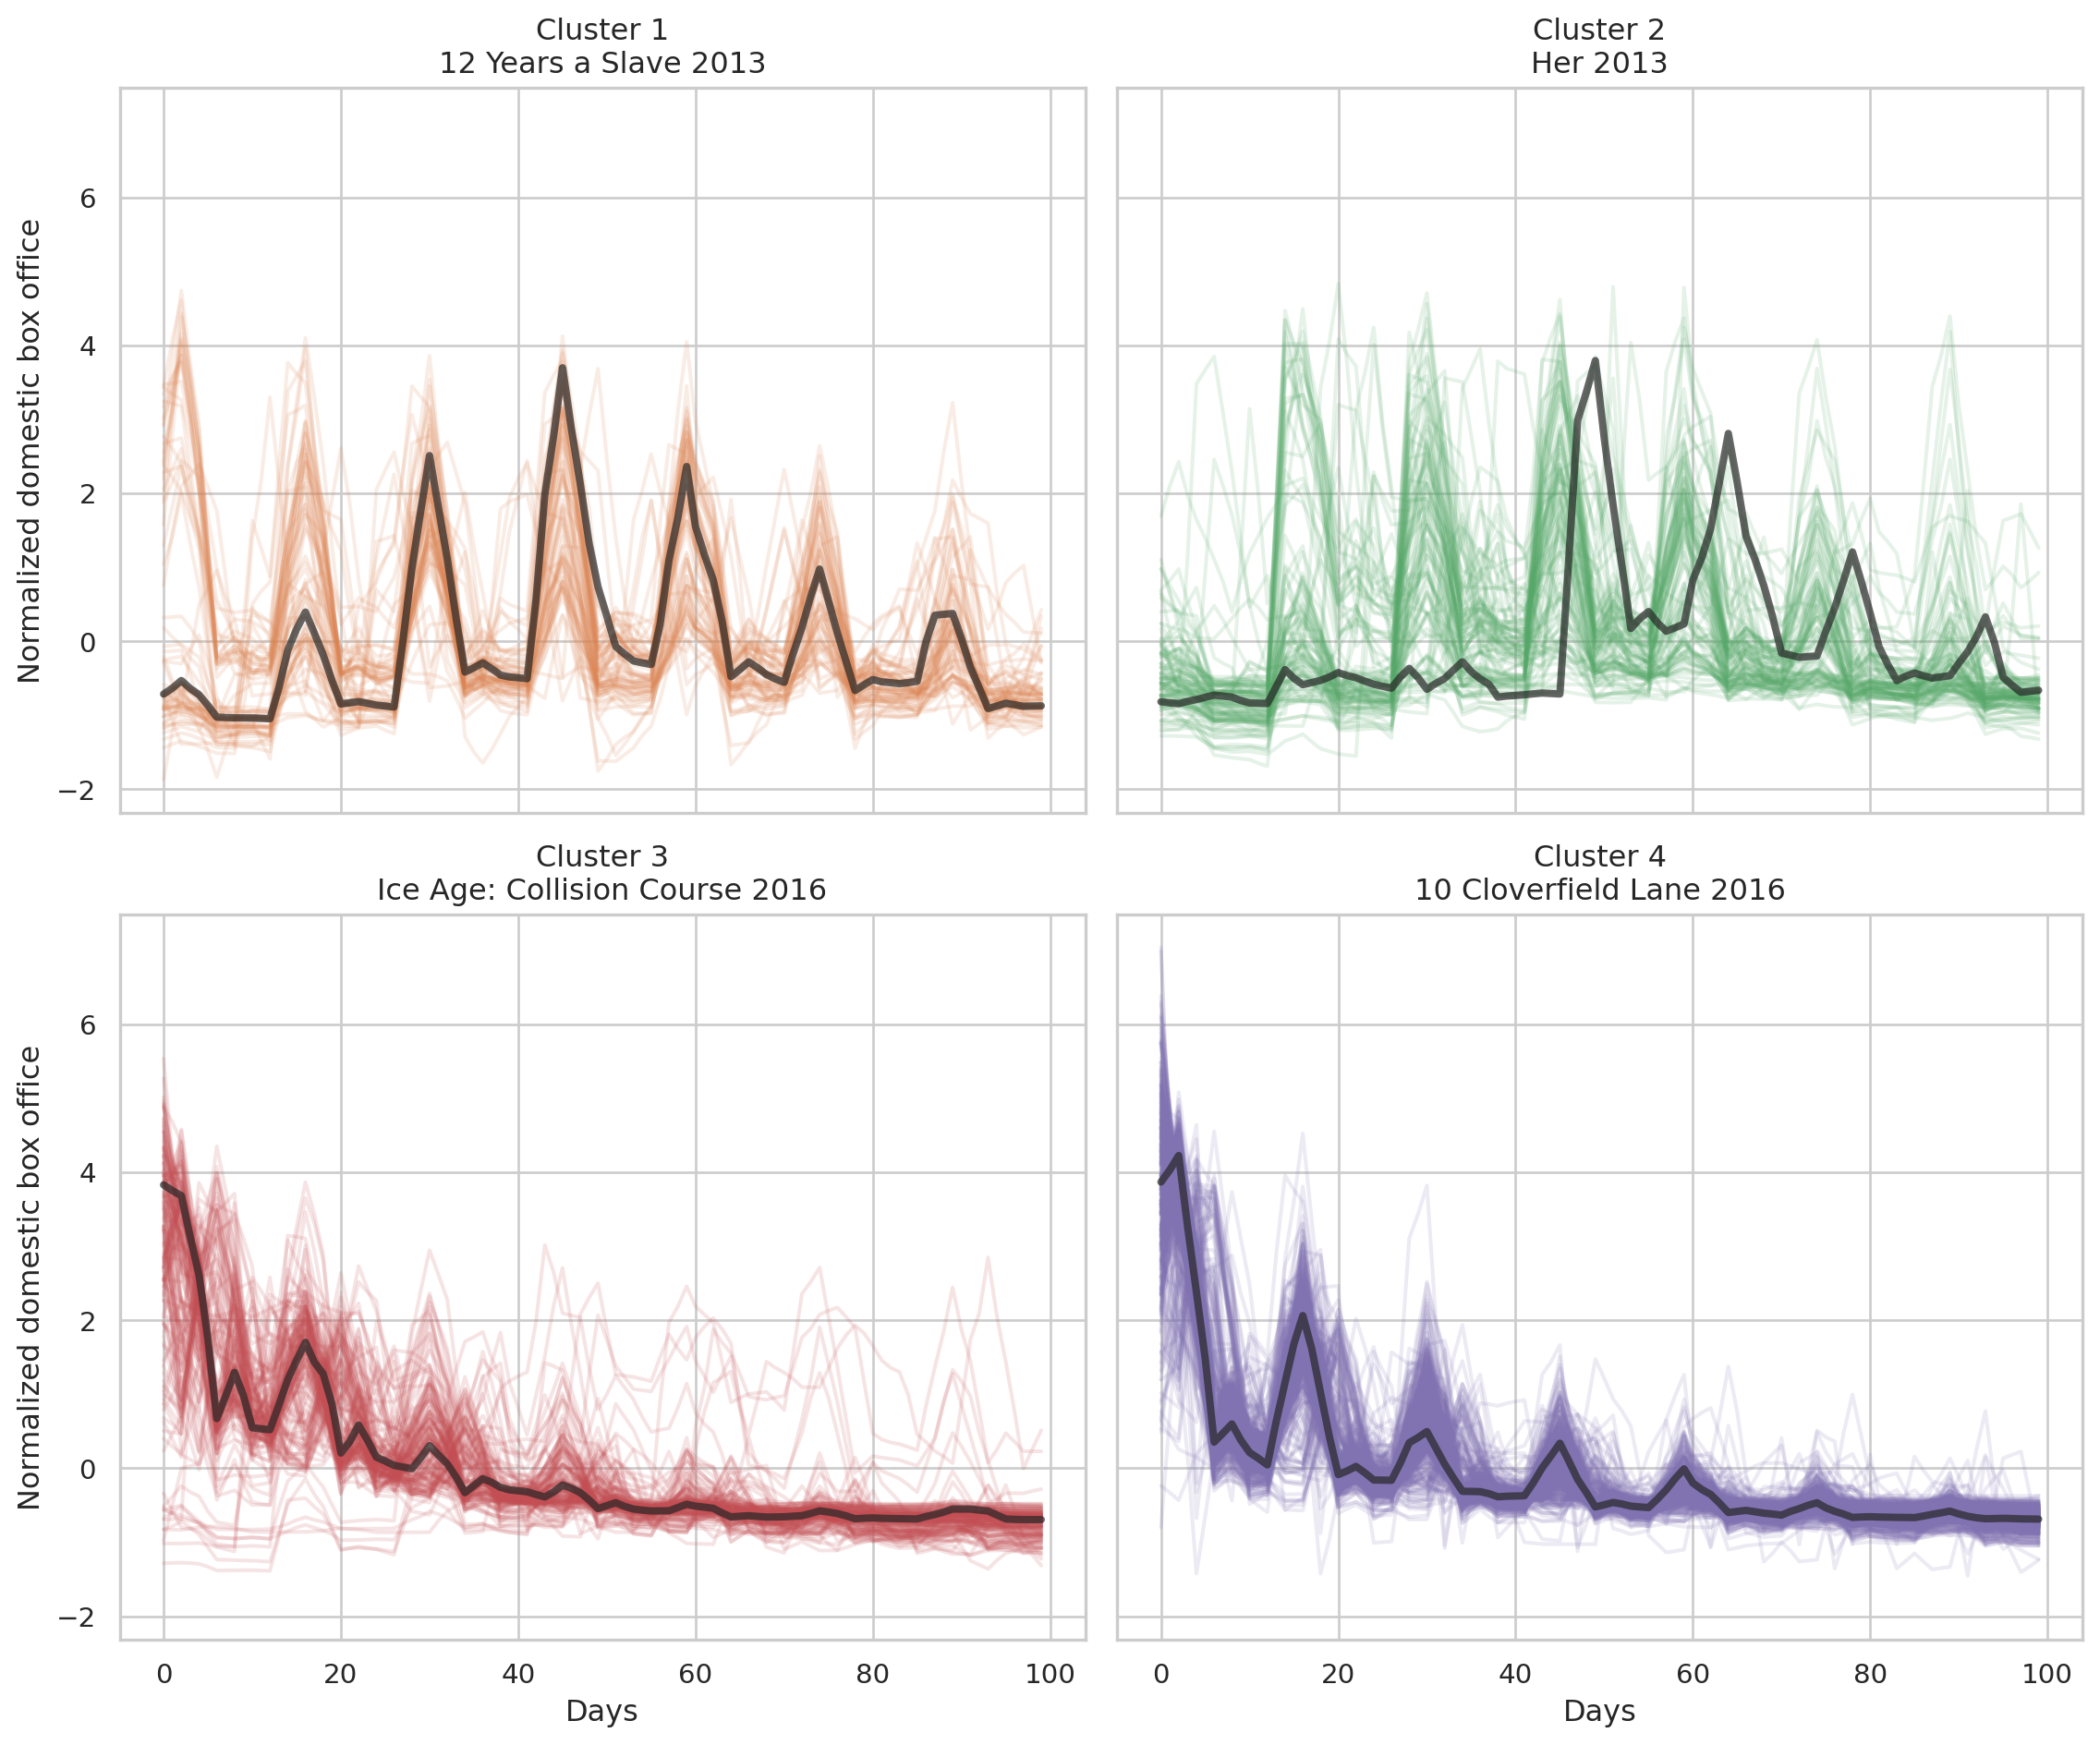
\includegraphics[width=\columnwidth]{../results/images/tsclust_structure.png}
    \caption{Clusters obtained by hierarchical clustering on structural features and respective cluster medoids (in black).}\label{fig:tsclust_structure.png}
\end{figure}

Analysis of clusters w.r.t. exogenous features showed very similar patters to those already observed in terms of rating, binned rating, awards, nominations, distribution of action and dramatic movies.



\end{document}
